\documentclass[11pt]{article}
\usepackage[T1]{fontenc}
\usepackage[utf8]{inputenc}
\usepackage{lmodern,microtype}
\usepackage[margin=1in,headheight=15pt]{geometry}
\usepackage{amsmath,amssymb,amsthm,mathtools}
\usepackage{booktabs,longtable,array,tabularx}
\usepackage{xcolor,graphicx,enumitem,fancyhdr,etoolbox}
\usepackage{listings}
\usepackage[colorlinks=true,linkcolor=navy,citecolor=teal,urlcolor=teal]{hyperref}
\definecolor{navy}{HTML}{17324D}
\definecolor{teal}{HTML}{087E8B}
\definecolor{muted}{HTML}{526477}
\definecolor{papergray}{HTML}{F1F5F8}
\newtheorem{theorem}{Theorem}[section]
\newtheorem{lemma}[theorem]{Lemma}
\newtheorem{proposition}[theorem]{Proposition}
\newtheorem{corollary}[theorem]{Corollary}
\theoremstyle{definition}
\newtheorem{definition}[theorem]{Definition}
\newtheorem{example}[theorem]{Example}
\theoremstyle{remark}
\newtheorem{remark}[theorem]{Remark}
\DeclareMathOperator{\supp}{supp}
\DeclareMathOperator{\poly}{poly}
\DeclareMathOperator{\rank}{rank}
\newcommand{\N}{\mathbb N}
\newcommand{\Z}{\mathbb Z}
\newcommand{\Q}{\mathbb Q}
\newcommand{\R}{\mathbb R}
\newcommand{\code}[1]{\texttt{\small #1}}
\newcommand{\status}[1]{\textsf{#1}}
\newcommand{\Reach}{\mathcal R}
\newcommand{\basecommit}{\texttt{66098968e88bba797143ac1bf7ad0ac4c5f697df}}
\setlength{\parskip}{0.35em}
\setlength{\parindent}{1.1em}
\setlist{itemsep=0.2em,topsep=0.35em}
\pagestyle{fancy}
\fancyhf{}
\fancyhead[L]{\small\color{muted}ProveIt research continuation}
\fancyhead[R]{\small\color{muted}Pachner traces and exact LP witnesses}
\fancyfoot[C]{\thepage}
\renewcommand{\headrulewidth}{0.3pt}
\lstset{basicstyle=\ttfamily\footnotesize,breaklines=true,
  backgroundcolor=\color{papergray},frame=single,rulecolor=\color{papergray},
  columns=fullflexible,keepspaces=true,showstringspaces=false}
\BeforeBeginEnvironment{lstlisting}{\par\noindent\begin{minipage}{\linewidth}}
\AfterEndEnvironment{lstlisting}{\end{minipage}\par}
\hypersetup{pdftitle={Single-Exponential Pachner Search and Exact Witness Reuse for Unknot Recognition},
 pdfauthor={Research report prepared for Vladimir Reshetnikov}}

\begin{document}
\hypersetup{pageanchor=false}
\begin{titlepage}
\vspace*{1.2cm}
{\color{teal}\large PROVEIT / TOPOLOGY / UNKNOT RECOGNITION\par}
\vspace{0.6cm}
{\color{navy}\Huge\bfseries Single-Exponential\par Pachner Search\par}
\vspace{0.3cm}
{\color{navy}\LARGE and Exact Witness Reuse\par for Unknot Recognition\par}
\vspace{0.9cm}
{\large A complete bounded search, a locality theorem,\par
and independently checked algorithmic improvements\par}
\vspace{0.8cm}
Research report prepared for Vladimir Reshetnikov\par
9 October 2026\par
\vfill
\noindent\textbf{Main result.} Bounded-upward geometric reachability can be searched in
$2^{O(t+U)}\poly(t+U+B)$ time. When the consumed initial tetrahedra lie in an allowed
region of size at most $r$ with at most $c$ connected components, the bound becomes
$t^c2^{O(r+U)}\poly(t+U+B)$. These bounds include a polynomial complete
endpoint predicate; a more expensive predicate must be charged separately.

\medskip
\noindent\textbf{Scope.} These are proved bounds for a precisely specified family of
formal Pachner replacements and transported cocycles. The report does not establish
a general quasi-polynomial unknot recognizer. The missing universal locality and
coverage theorem is stated explicitly.

\medskip
\noindent\textbf{Source revision.}\par
\small\basecommit\par
\noindent Three incoming research archives are reviewed and preserved as dependencies.
\end{titlepage}
\hypersetup{pageanchor=true}
\pagenumbering{roman}

\begin{abstract}
We replace unrestricted enumeration of local-move orderings by a complete
search based on the eventual use of each tetrahedron. Every tetrahedron incarnation
has eleven possible commitments: remain unused, be consumed at one of six edges
by a $3$--$2$ move, or be consumed at one of four faces by a $2$--$3$ move.
Consistently committed enabled moves have disjoint supports and commute. Any trace
with at most $U$ upward moves is equivalent to a deterministic committed execution;
at most $3t+5U$ incarnations are involved. Consequently bounded-upward marked
reachability admits a single-exponential search. An exact sleep-set implementation
inherits this bound while avoiding the large overhead of enumerating inert
commitments. A reverse-search generator for regions in the degree-four initial
dual graph sharpens the bound to $t^c2^{O(r+U)}$ when an allowed region has at most
$r$ tetrahedra and $c$ components. This gives a constructive quasi-polynomial
search class for $c=O(\log t)$ and $r+U=O(\log^2 t)$.

Separately, exact positive witnesses screen redundant deletion queries in
normal-surface LP propagation. Minimal support antichains preserve every completed
certificate of the deterministic baseline. An explicit algebraic family reduces
LP calls from $3s^2+2s+1$ to $2s+1$ and exact simplex pivots from
$6s^3+3s^2+s$ to $3s^2+s$. The artifact contains additive code, independent
replay, genuine triangulation controls, paired measurements, and a diagram-bound
positive-certificate adapter. Exhaustion of a bounded coherent family is never
reported as knottedness. The results improve concrete search and propagation
operations, and identify the geometric statement still needed for a general
quasi-polynomial recognition guarantee.
\end{abstract}

\begingroup
\small
\setlength{\parskip}{0pt}
\tableofcontents
\endgroup
\clearpage
\pagenumbering{arabic}
\section{What this continuation establishes}

The principal improvement concerns discovery. Given a triangulation, a fixed
integral cocycle, and a bound on the total number of expanding Pachner moves,
the new search covers every permitted finite trace up to explicit marked
combinatorial isomorphism. Its analysis removes an unnecessary $\log t$ factor
from the exponent of naive move-string enumeration. More significantly, it
allows a locality parameter to replace the full initial tetrahedron count in
the exponential factor. The normal-surface LP improvement is independent and
can be enabled without changing the mathematical branch policy.

\begin{center}
\small
\begin{tabularx}{\textwidth}{@{}l>{\raggedright\arraybackslash}X>{\raggedright\arraybackslash}X@{}}
\toprule
Result & Proved guarantee & Remaining restriction\\
\midrule
Commitment encoding & At most $11^{3t+5U}$ encodings of bounded-upward trace classes & $U$ counts total upward moves\\
Sleep-set exploration & One explored representative per commuting trace class & Precise local action identities are required\\
Region search & $t^c2^{O(r+U)}\poly(t+U+B)$ with a polynomial complete endpoint predicate & A small region must contain the successful initial footprint\\
LP witness screening & Same completed baseline certificate; fewer deletion LPs & Node LPs and the search tree can remain expensive\\
Source-bound adapter & Every \status{UNKNOT} has independent geometric replay & A failed bounded search is inconclusive\\
\bottomrule
\end{tabularx}
\end{center}

These statements concern operations that are implemented in the accompanying
artifact. Their proofs do not assume that an observed success rate extends to
all unknots. Nor does the reported single-exponential bound improve the best
general exponential classification of unknot recognition. It improves a
particular geometric search mechanism and supplies a sharper constructive
condition under which that mechanism is quasi-polynomial.

\subsection{Pinned repository and the incoming work}

The source audit is pinned to the GitHub main revision
\begin{center}\small\basecommit.\end{center}
The relevant maintained directory is
\path{Topology/UnknotRecognition}; the three incoming archives are in
\path{docs/incoming}. Their Git object identities and SHA-256 digests are
retained in the package provenance. Source files were obtained from this
immutable revision, not from a moving working-tree comparison.

The incoming dual-certificate report supplies exact positive-Euler LP
propagation, dual replay, and primitive-ray certificates. Its search still
restarts a rational LP for every unskipped deletion test. The geometric-transport
report supplies formal Pachner moves, signed cocycle transport, local scores,
and a diagram-bound disc verifier, but implements a single deterministic
downward epoch. The support-sensitive report supplies more economical
component and rank-one certificates. Its contributions are retained for
reproduction but are not presented as new results here.

\begin{center}
\small
\begin{tabularx}{\textwidth}{@{}lX@{}}
\toprule
Incoming archive & Dependency relevant to this continuation\\
\midrule
\path{unknot_dual_certificates_20261009.zip} & Exact kernel LP, standard-coordinate propagation and independent proof checker\\
\path{unknot_geometric_transport_20261009.zip} & Cochain transport, geometric score controls and diagram-bound terminal verification\\
\path{unknot_support_sensitive_certificates_20261009.zip} & Support and component certificate infrastructure; reviewed separately from the new claims\\
\bottomrule
\end{tabularx}
\end{center}

The public repository's current source and these incoming artifacts are
unpublished project material \cite{ProveIt,DualIncoming,TransportIncoming,SupportIncoming}.
The additive overlay avoids rewriting their existing production functions.
The supplied integration script accepts an already present byte-identical
dependency and refuses a conflicting file, so a later integration can be
reviewed against the pinned baseline.

\subsection{Relation to the published and announced algorithms}

Lackenby's 109-page 2021 talk announces an $n^{O(\log n)}$ unknot-recognition
algorithm and describes multi-surfaces and Cheeger-region reductions
\cite{LackenbyTalk}. The July 2026 paper develops a hierarchy algorithm for
incompressibility. Its Proposition 9.1 bounds hierarchy-loop work by
$L(g+1)^L$; the refined length bound is linear in a decomposition complexity.
The paper does not provide the complete quasi-polynomial implementation sought
here \cite{Lackenby2026}. A separate compressed Oxford handout uses a different
displayed exponent, so the artifact identifies the exact talk version it cites.

Pachner-graph search and partial commutation of moves have substantial prior
work. Burton studies simplification paths and explicitly rearranges certain
consecutive moves, including overlapping composite cases
\cite{BurtonPachner}. Burton and He prove an existence theorem for unimodal
elementary-move sequences \cite{BurtonHeMoves}. Our proof uses a smaller
independence relation---disjoint consumed tetrahedra---and obtains an explicit
bound in the total upward count and initial region. No claim is made to have
introduced commutation to triangulation algorithms or to dominate every
existing Pachner-graph implementation.

Sleep sets are a standard partial-order verification technique
\cite{Godefroid}. The new argument specializes their required independence
conditions to the repository's exact formal replacements and combines them
with the incarnation count. The LP baseline belongs to the normal-surface
branching tradition developed, for example, by Burton and Ozlen
\cite{BurtonOzlen}. The abstract hardness result of Burton and He cautions
against inferring an easy general normal-surface search from its linear
relaxation \cite{BurtonHeHardness}.

\subsection{What counts as evidence}

There are three separate standards throughout this report. A mathematical
theorem has an explicit model and proof. A correctness claim about the code
has independent replay or comparison with an independent finite oracle.
A performance claim has a declared workload, caps, raw timings and a paired
comparison. These standards answer different questions. A short execution on
the coherent obstruction does not prove a universal small-footprint theorem;
a factorial operation-count separation does not guarantee that validation
overhead is negligible; a completed LP proof does not authenticate a knot
diagram unless source geometry is also included.

\section{The geometric search model}\label{sec:model}

\subsection{Face-paired triangulations and legal replacements}

A triangulation is a finite list of abstract tetrahedra with local vertices
$0,1,2,3$. Each triangular face is either a boundary face or is paired to
another face by a full vertex permutation. Global vertices and edges may
have multiple local representatives. The existing validator checks the
manifold and matching requirements of the normal-surface interfaces.
This is the usual generalized triangulation setting used in computational
three-manifold topology, rather than a requirement that every global vertex
set specify a unique simplex \cite{BurtonPachner}.

A legal $2$--$3$ replacement consumes two distinct tetrahedra sharing a face.
Their formal union is a triangular bipyramid. It is replaced by the three
tetrahedra around the other diagonal, preserving all six labelled boundary
facets and their attaching permutations. A legal $3$--$2$ replacement consumes
three distinct tetrahedra constituting the entire degree-three star of an
interior edge, with the formal triangular-link consistency checked by the
existing producer. It performs the inverse relative-boundary replacement.

These conventions are substantive. All independence statements below use the
repository's formal-bipyramid legality. If one additionally imposed strict
simplicial-complex conditions forbidding a new edge or face already present
elsewhere, disjoint consumed supports would require a fresh independence
analysis. The source code does not silently switch between these conventions.

\begin{definition}[Incarnation and event]
A tetrahedron incarnation is one specific tetrahedron from its creation until
its destruction. An event is a legal replacement together with the identities
of all consumed incarnations and the local edge or face selected in each.
Surviving incarnations keep their local vertex labels; replacement outputs
receive new identities and the canonical local labels of the producer.
\end{definition}

An incarnation is not a row number. After deleting three rows, a survivor's
row number can change even though its identity, local corners and commitment
remain unchanged. The implementation keeps this distinction explicit.

\subsection{Cocycles and the endpoint surface}

The input marking is a list of four integral heights $h_{t,0},\dots,h_{t,3}$
per tetrahedron. The signed differences on identified edges must agree; they
therefore define an integral cocycle. Adding a constant to one height row
does not change the marking. The implementation normalizes each row by
subtracting its first entry.

For bit-complexity statements, $B$ bounds the bit lengths of both the supplied
height entries and their edge differences. If rows are already normalized,
the edge data alone suffice. Including the supplied entries charges the
input-reading and normalization cost even when a row has an unnecessarily
large additive constant.

If $a,b,c,d$ order the corners so that
$h_a\le h_b\le h_c\le h_d$, the corresponding coherent normal vector has
triangle coordinates $h_b-h_a$ at $a$ and $h_d-h_c$ at $d$, and the single
quadrilateral coordinate $h_c-h_b$ separating $\{a,b\}$ from $\{c,d\}$.
All other local coordinates vanish. Ties cause zero coordinates and cause no
ambiguity in the resulting normal vector.

The five formal bipyramid heights determine the transported cocycle on the
new tetrahedra. This preserves the global cohomology class. It can change the
topology of the coherent normal surface: the incoming transport package gives
a checked example in which a disc becomes a disc and two spheres. Thus raw
Euler characteristic is not used as a terminal unknot criterion.

\begin{definition}[Bounded-upward family]
For a source $(T,h)$ and integer $U\ge0$, let $\Reach_U(T,h)$ be the marked
endpoints of all finite legal $2$--$3$/$3$--$2$ traces containing at most $U$
\emph{total} $2$--$3$ events, with the prescribed cocycle transport at every
event. The empty trace and all intermediate endpoints are included.
\end{definition}

If a trace contains $u$ upward and $d$ downward events, its tetrahedron count is
\begin{equation}\label{eq:tet-account}
 t'=t+u-d.
\end{equation}
In particular, $d\le t+u$ and the trace length is at most $t+2U$. The maximum
tetrahedron count is at most $t+U$. These coarse inequalities also cover
degenerate stopping points without requiring a special minimum-size constant.

The parameter $U$ is different from the maximum excess tetrahedron count and
from the number of upward bursts. Repeated expansion--collapse pairs can have
excess height one and arbitrarily many upward events. Our completeness proof
permutes independent upward and downward events; it preserves total counts,
but does not preserve every prescribed burst pattern.

\begin{center}
\begin{tabular}{@{}ll@{}}
\toprule
Symbol & Meaning\\
\midrule
$n$ & Number of crossings when a knot diagram is the original input\\
$t$ & Number of tetrahedra in the source of one geometric search\\
$U$ & Allowed total number of $2$--$3$ events\\
$F,r$ & Allowed set of original tetrahedra and its size bound\\
$c$ & Maximum number of connected components of the allowed region\\
$B$ & Initial bit-length bound including supplied heights and edge values\\
$Q$ & Number of outer searches in a conditional recognition analysis\\
\bottomrule
\end{tabular}
\end{center}

\subsection{Endpoints, traces and decision predicates}

Two adjacent events with disjoint consumed supports will be shown to commute.
Trace equivalence is generated by such adjacent interchanges, carrying local
labels and the marking through the induced isomorphisms. Endpoint predicates
must respect this transported isomorphism. The existence of an essential-disc
component does; a predicate inspecting the arbitrary order of rows in a
certificate need not.

The code supports an arbitrary callback for experimentation, but
\status{ENDPOINT\_SELECTED} means only that this callback selected a supplied
state. A \status{DISC\_FOUND} result additionally carries an independently
checked component-disc proof. Source geometry is then needed to turn the latter
into \status{UNKNOT} for a given diagram.

\section{Commitments and the single-exponential bound}\label{sec:commitments}

\subsection{The relative-boundary commutation lemma}

\begin{lemma}[Commuting disjoint supports]\label{lem:commute}
Let $a,b$ be simultaneously legal formal replacements in a triangulation,
and suppose that their sets of consumed tetrahedron incarnations are disjoint.
After applying $a$, the transported event $b$ remains legal; the symmetric
statement holds. The results of $ab$ and $ba$ have a canonical combinatorial
isomorphism fixing every surviving old tetrahedron and respecting the two
replacement regions, their boundary attachments and their transported cocycles.
\end{lemma}
\begin{proof}
Regard each consumed region as a separate formal bipyramid before the global
face identifications. Both fillings have the same labelled six-facet boundary.
One can replace both fillings simultaneously and then impose the original
attaching maps. Replacing them in either order gives exactly this quotient.
This also covers the case that a boundary face of one region is attached to
a boundary face of the other: the common attaching permutation is retained
in the simultaneous construction.

The internal face of a $2$--$3$ event belongs to its two consumed tetrahedra.
The complete central-edge star of a $3$--$2$ event belongs to its three
consumed tetrahedra. A disjoint replacement changes neither of these internal
configurations. Its updates to exterior attachments merely apply the same
relative-boundary identifications. Hence the second event stays legal.

For the marking, the five heights in each formal region are reconstructed
from the same old edge differences. Changes of additive row constants have
no effect. The regions use disjoint old tetrahedron interiors and retain the
same boundary edge values. The two independently obtained sets of new rows
therefore agree after the stated isomorphism and normalization. No claim
that the intermediate coherent surfaces have identical topology is required.
\end{proof}

Disjoint support is sufficient, not necessary. Overlapping moves can also
have special relations, as in the earlier Pachner-graph literature
\cite{BurtonPachner}; the present proof deliberately requires only the
uniformly checked relation in Lemma~\ref{lem:commute}.

\subsection{A constant alphabet on each incarnation}

Assign an incarnation one of the following eleven symbols:
\[
 \mathcal A=\{\text{idle}\}
 \cup\{\text{down at edge }e:0\le e<6\}
 \cup\{\text{up at face }f:0\le f<4\}.
\]
The six edges use a fixed ordering of the pairs of local vertices.
An enabled downward event is \emph{ready} if all three source incarnations
are committed to their local copy of its central edge. An upward event is
ready if both source incarnations are committed to the common face. Upward
events are disabled when the total upward budget is exhausted.

\begin{lemma}[Ready events cannot compete]\label{lem:ready}
Two different ready events consume disjoint sets of incarnations.
\end{lemma}
\begin{proof}
A shared incarnation would have to select the same symbol for both events.
The idle symbol selects no event. A selected local face identifies its unique
partner and hence its unique $2$--$3$ event. A selected local edge identifies
its entire global edge star and hence the unique legal $3$--$2$ event at
that edge. Thus the purported events would be equal.
\end{proof}

The committed search uses a fixed deterministic order of ready events. If
one exists, it executes the first, preserves commitments on survivors and
leaves new incarnations unassigned. If none exists, it assigns the first
unassigned live incarnation one of the alphabet symbols, branching on every
choice. If none is unassigned, that branch stops. An assignment need not be
consistent with any eventual move; inert assignments are allowed and counted.

The implementation evaluates a state predicate at each newly encountered
marked endpoint, before deciding whether to continue. This avoids the extra
assumption that a useful surface survives every later downward choice.

\begin{theorem}[Complete commitment encoding]\label{thm:commitment}
Let $T$ have $t$ tetrahedra and let $U\ge0$. Every permitted trace defining
an endpoint in $\Reach_U(T,h)$ is equivalent to an execution of the
deterministic committed scheduler.
At most $3t+5U$ incarnation symbols are needed. Consequently the number of
commuting trace classes, including classes of all finite prefixes, is at most
\begin{equation}\label{eq:commitment-count}
 11^{3t+5U}.
\end{equation}
For $U=0$, the alphabet can be restricted to seven symbols and the corresponding
bound is $7^{3t}$.
\end{theorem}
\begin{proof}
Fix a target finite trace. For each incarnation appearing in it, record the
local port of the event that eventually consumes it; if it survives to the
target endpoint, record idle. Follow these assignments in the deterministic
scheduler, interpreting them under the transported local labels.

Suppose an event is currently ready. Consider the first event in the
remaining target trace that touches one of its source incarnations. Until
that first touch, the ready event's common face or full central-edge star is
unchanged. The touched incarnation's commitment specifies the local port of
its eventual consuming event. This is the ready event's port, so uniqueness
at that port implies that the first touching event is exactly the ready
event. All earlier target events have disjoint consumed supports. By
Lemma~\ref{lem:commute}, the ready event can be moved to the front across all
of them. This interchange preserves the endpoint, the marking and the total
upward count. Its new prefix cannot exceed the total allowed upward count.

If no event is ready, assign the next unassigned incarnation its recorded
symbol. Once the participants of the first remaining target event have
received their symbols, that event is ready. Thus this process cannot stop
before all target events have been performed, apart from harmless
reordering. All target survivors are idle, so it stops at the required
endpoint after the assignments are completed. This proves completeness and
trace equivalence without asserting confluence of uncommitted downward
rewriting.

If the execution has $u$ upward and $d$ downward events, the total number of
incarnations is
\[
 N=t+3u+2d\le t+3u+2(t+u)=3t+5u\le3t+5U.
\]
Each is assigned at most once. Encode the assignments in the deterministic
order in which the scheduler requests them, and pad a shorter encoding to
length $3t+5U$ by idle symbols. Replaying a word determines one execution.
If two trace classes had the same encoding, they would both commute to
that same execution and would be equal. Hence there are at most the number
of such words. The same construction applied to any target prefix, giving
its survivors idle, proves the assertion for all prefix classes. Omitting
upward symbols gives the last statement.
\end{proof}

\begin{remark}[Assignments are not geometric steps]
The encoding algorithm is a proof device as well as a reference implementation.
Many assignments lead nowhere. Its tree has at most
$(11^{N+1}-1)/10$ assignment vertices, with polynomially many forced-move
operations along an assignment path. It can be much slower on a small
triangulation than direct trace reduction. The bound does not justify a
claim of practical speed by itself.
\end{remark}

\subsection{Sleep sets give an efficient realization of the same bound}

At a search node maintain a set of sleeping event identities. Explore the
enabled events in deterministic order. Skip a sleeping event. After exploring
an event $a$, add $a$ to the local sleep set for later sibling branches.
For a child reached by $b$, retain only sleeping events whose consumed support
is disjoint from $b$'s support. Thus an event is remembered across a replacement
exactly when the proved commutation rule permits it to move past that replacement.

\begin{theorem}[Sleep-set coverage and uniqueness]\label{thm:sleep}
With exact incarnation identities, one canonical event per eligible edge or
face, and the independence relation of Lemma~\ref{lem:commute}, sleep-set
exploration visits at most one representative of each commuting trace class.
Every reachable marked endpoint has a visited representative. Hence the
number of visited trace nodes is at most $11^{3t+5U}$, or $7^{3t}$ when $U=0$.
\end{theorem}
\begin{proof}
For uniqueness, suppose equivalent traces first diverge at a state where the
earlier branch takes $a$ and a later branch takes $b$. The later branch starts
with $a$ sleeping. Legal interchanges preserve exact event identities, so it
must eventually perform that same event $a$. None of its consumed
incarnations can have been destroyed in the intervening prefix: an
incarnation never reappears after destruction. Every intervening event thus
has consumed support disjoint from $a$. Initially $a$ is enabled, and
Lemma~\ref{lem:commute} inductively keeps it enabled across that prefix.
The sleep-update rule retains $a$ throughout, so its eventual occurrence is
forbidden. This is a contradiction.

For coverage, choose among the finitely many representatives of any target
trace class the first one in the deterministic search order. If it were
blocked by a sleeping event, the earlier occurrence that put that event to
sleep could be commuted across the intervening independent events, giving
an earlier representative of the same class. This contradicts the choice.
Equivalently, repeatedly move the earliest blocking event left until no
blocking event remains; the finite lexicographic order decreases. Thus
the chosen representative is visited. Lemma~\ref{lem:commute} supplies
the persistence of all transported enabled events used in this argument.

The total-upward restriction is invariant under these interchanges. Protected
initial cells, when present, are also invariant. Apply
Theorem~\ref{thm:commitment} to the resulting representatives.
\end{proof}

This proof uses the standard sleep-set principle \cite{Godefroid}, but its
hypotheses are checked for these geometric events. The implementation does
not merge search continuations merely because their raw triangulations agree.
Different remaining upward budgets and sleep sets can permit different
continuations. A separate exact state table suppresses repeated endpoint
queries only; exploration continues from every scheduled state.

Independence here concerns simultaneously enabled events, or legal adjacent
interchanges. It is not a static relation inferred only from the consumed
sets of arbitrary historical events: a later event can consume an output
born from an earlier event even though their consumed sets are disjoint.
The persistence and nonresurrection argument above is what justifies the
actual sleep update.

\subsection{A genuine factorial-to-subset separation}

Suppose $p$ independent downward events are enabled, no other downward event
is created, and each can be executed at most once. Unreduced all-prefix
enumeration visits
\begin{equation}\label{eq:factorial}
 N_{\rm naive}(p)=\sum_{j=0}^{p}\frac{p!}{(p-j)!}
 =p!\sum_{k=0}^{p}\frac1{k!}.
\end{equation}
Every subset of events is a distinct prefix endpoint and all orderings of
that subset commute. Sleep exploration visits exactly $2^p$ nodes. Full
maximal orders alone are reduced from $p!$ to one.

The artifact realizes this situation by disjoint inverse bipyramids in a
layered solid torus and verifies the move inventory and endpoints. It is
therefore an actual geometric control. Equation~\eqref{eq:factorial} is a
proof under its stated event-inventory hypothesis; finite tests of the
construction are reported at the tested sizes. We do not extrapolate the
measured construction to a universal claim about all solid-torus
triangulations.

\section{Locality replaces the full tetrahedron count}\label{sec:regions}

The uniform commitment bound still has an exponent linear in $t$, even when
only a small part of a triangulation participates in a useful sequence. The
next result charges the exponent to the \emph{initial} region that the trace
is allowed to consume. Newly created tetrahedra are included automatically
in the incarnation accounting.

\begin{definition}[Allowed initial region]
Let $G_T$ be the simple graph on the original tetrahedra, with adjacency when
they share a paired face. An allowed initial region is a set
$F\subseteq V(G_T)$. A trace is supported in $F$ if no original tetrahedron
outside $F$ is consumed. It may consume every subsequently created tetrahedron.
For $r,c,U\ge0$, let $\Reach_{r,c,U}(T,h)$ be the union of bounded-upward
families supported in regions $F$ with $|F|\le r$ and at most $c$ connected
components in $G_T[F]$.
\end{definition}

We use effective integer caps $0\le r\le t$ and $0\le c\le r$;
larger supplied caps can be reduced to these values without changing the
family. The empty region is included, so zero caps still allow the source
endpoint to be checked.

The region is a \emph{cover} of the actual initial consumption footprint.
Some members of $F$ may survive. An actual consumed set can have several
components while lying inside one connected allowed region. This distinction
matches the executable search and is useful when a small connecting corridor
is included in the supplied region.

\subsection{A supplied region}

\begin{theorem}[Region-sensitive commitment bound]\label{thm:fixed-region}
For a supplied region $F$ of size $i$, the family supported in $F$ with at
most $U$ upward events has at most $11^{3i+5U}$ commuting trace classes.
When $U=0$, the bound is $7^{3i}$. Both the commitment search and the sleep
search exhaust this family with polynomial overhead per encoding or
representative, apart from endpoint-predicate work.
\end{theorem}
\begin{proof}
Give every original tetrahedron outside $F$ the forced symbol idle. Such
tetrahedra are protected forever. After $u$ upward and $d$ downward events,
at least $t-i$ original tetrahedra remain, so
\[
 t+u-d\ge t-i,\qquad d\le i+u.
\]
Only the $i$ initially eligible tetrahedra and all newly born tetrahedra need
freely chosen commitments. Their number is
\begin{equation}\label{eq:active-incarnations}
 i+3u+2d\le3i+5u\le3i+5U.
\end{equation}
The proof of Theorem~\ref{thm:commitment} preserves the identities of consumed
original tetrahedra under every interchange, so it remains valid with the
protection restriction. The sleep-set proof also preserves this restriction.
Every generated trace is supported in $F$, and every trace supported in $F$
has its prescribed idle commitments on the protected originals.
\end{proof}

The number of events in such a trace is at most $i+2U$, even when the
surrounding triangulation is much larger. The code checks the two inequalities
in this proof at every search frame. A bad bookkeeping update therefore
cannot silently invalidate the claimed measure.

\subsection{Counting and enumerating regions}

The maximum number of distinct neighbours of a vertex of $G_T$ is four.
Loops and repeated face adjacencies do not increase this bound.

\begin{lemma}[Counting connected regions]\label{lem:connected-count}
In a graph with $t\ge1$ vertices and maximum degree at most four, the number
of connected $i$-vertex subsets is at most $t16^{i-1}$ for $i\ge1$.
The number of subsets of size at most $r$ with at most $c$ connected
components, including the empty set, is at most
\begin{equation}\label{eq:region-count}
 (r+1)(c+1)t^c32^r.
\end{equation}
\end{lemma}
\begin{proof}
Root a connected set at its least-labelled vertex. Choose a deterministic
spanning tree of the induced graph and traverse its edges depth first,
each twice. Record the root and the chosen local neighbour port at each
of the $2(i-1)$ steps. There are at most four choices at each step. The
walk reconstructs the visited vertex set, so the encoding is injective
on the connected sets selected by the deterministic rule. This proves
$t4^{2(i-1)}$.

For a set of size $i$ with $j\ge1$ components, order the components by their
least vertex. Encode their $j$ roots, their positive sizes summing to $i$,
and their walks. This gives the upper bound
\[
 t^j\binom{i-1}{j-1}16^{i-j}\le t^j32^i.
\]
Summing over $1\le i\le r$ and $1\le j\le\min(c,i)$, then adding the empty
set, proves the intentionally coarse uniform bound
\eqref{eq:region-count}. It also holds for $r=0$ or $c=0$.
\end{proof}

Counting alone would not give a useful algorithm if finding those regions
required enumerating all $t^r$ subsets. The artifact uses the following
explicit reverse search.

\begin{lemma}[Canonical parent and complete reverse search]\label{lem:reverse}
For a connected set $A$ with root $\rho=\min A$ and $|A|>1$, delete the
largest $x\in A\setminus\{\rho\}$ for which $G_T[A\setminus\{x\}]$ stays
connected. This defines a unique parent. Starting from every singleton,
and accepting an added frontier vertex precisely when this rule returns
the current set as parent, enumerates each connected region once, with
polynomial overhead in its size.
\end{lemma}
\begin{proof}
A spanning tree of $G_T[A]$ has a leaf other than $\rho$. Deleting that leaf
leaves a spanning tree on the other vertices, hence preserves connectivity
of the induced graph. At least one eligible deletion therefore exists.
The largest-label rule makes it unique. Iterating the parent decreases
size and preserves the root, eventually reaching $\{\rho\}$.

Any child of $A$ adds a vertex adjacent to $A$: otherwise it is not connected.
The algorithm therefore considers it among the frontier vertices and accepts
it at its unique parent. It cannot be accepted at another parent. There are
at most $4|A|$ distinct frontier candidates; each parent computation needs
at most $|A|$ connectivity tests on at most $|A|+1$ vertices. This is
polynomial overhead, with no enumeration of vertex-addition permutations.
\end{proof}

For several components, the code selects connected pieces in increasing
order of their least vertex. After choosing a component, it excludes its
closed neighbourhood from later components. The pieces are consequently
the actual components of the permitted region. Every allowed region has
exactly one such ordered decomposition. The same reverse-search argument
works in the remaining induced graph. An explicit stack avoids a recursion
limit tied to the number of vertices.

\subsection{The constructive locality theorem}

\begin{theorem}[Complete local reachability]\label{thm:local}
Let $(T,h)$ be a valid source with $t\ge1$ tetrahedra and initial cocycle
bit bound $B$. Suppose a chosen endpoint predicate is invariant under the
tracked marked isomorphisms and has polynomial bit complexity. Then
$\Reach_{r,c,U}(T,h)$ can be searched exhaustively in
\begin{equation}\label{eq:local-bound}
 t^c2^{O(r+U)}\poly(t+U+B)
\end{equation}
bit operations. A precise sufficient counting factor is
\[
 (r+1)(c+1)t^c32^r11^{3r+5U}.
\]
Every successful endpoint is geometrically replayable from the supplied
source. If the endpoint predicate has a different worst-case cost, that
cost must be included as an additional factor.
\end{theorem}
\begin{proof}
Enumerate the regions by Lemma~\ref{lem:reverse} and its component extension.
For each region use Theorem~\ref{thm:fixed-region}. The union is exactly the
defined family: membership requires containment in at least one such region.
Repeated endpoints across different regions do not affect correctness or
the upper bound. Lemma~\ref{lem:connected-count} bounds the number of regions.
The polynomial marking and geometric costs are established in
Section~\ref{sec:verification}. Multiplying these factors proves the claim.
\end{proof}

\begin{corollary}[Polynomial and quasi-polynomial classes]\label{cor:quasi}
For one connected allowed region, $r+U=O(\log t)$ gives a polynomial search
bound, and $r+U=O(\log^2 t)$ gives $t^{O(\log t)}\poly(B)$.
More generally, $c=O(\log t)$ together with $r+U=O(\log^2 t)$ gives the
latter quasi-polynomial bound.
\end{corollary}
\begin{proof}
Take logarithms of the non-polynomial factor in
\eqref{eq:local-bound}: it is $O(c\log t+r+U)$. Substitute the stated
conditions. The fixed polynomial factors do not change these classifications.
\end{proof}

This improves what a direct move-string analysis provides for the same
locality conditions. A trace has at most $r+2U$ events but can choose among
$O(t+U)$ locations at each event. That direct bound pays
$O((r+U)\log(t+U))$ in the exponent. The region theorem pays
$O(c\log t+r+U)$, isolating the cost of choosing the spatial components.
The improvement concerns the explicit search model, not a lower bound on
every alternative way to recognize knots.

\subsection{A precise remaining global obligation}

Suppose an outer, source-certified algorithm makes $Q(n)$ calls of this
kind on sources with parameters $t_i,B_i,r_i,c_i,U_i$. Its accumulated cost
is bounded by the sum of the individual costs, plus its other work:
\begin{equation}\label{eq:outer-sum}
 \sum_{i=1}^{Q(n)}t_i^{c_i}2^{O(r_i+U_i)}\poly(t_i+U_i+B_i).
\end{equation}
Thus polynomially bounded source sizes and markings, a quasi-polynomial
number of outer calls, and the bounds in Corollary~\ref{cor:quasi} would
yield a quasi-polynomial total. This is a sufficient accounting statement.
It does not prove completeness of such an outer algorithm or bound its
restarts. In particular, the existence of a short successful trace for an
unknot alone says nothing about how a negative instance is decided.

The outstanding geometric target is now concrete: establish a useful
small-region coverage theorem for a specified source construction and
surface family, including its behavior after certified reductions. The
existing coherent-height obstruction shows that coverage cannot be asserted
without allowing changes of triangulation or a richer surface representation.

\section{Bit complexity and the verification boundary}\label{sec:verification}

\subsection{Binary cocycle values stay controlled}

\begin{lemma}[Height growth under a bounded number of expansions]\label{lem:bits}
Let $D_0$ be the maximum absolute source edge value. After any trace with
$u$ upward events, every signed edge value has absolute value at most
$2^uD_0$. A normalized tetrahedral height row and every local coherent
normal coordinate have bit length at most $B+u+O(1)$ when $D_0<2^B$.
\end{lemma}
\begin{proof}
A downward replacement removes its central edge and creates no new global
edge. Surviving edge values are unchanged. For an upward replacement, the
new diagonal joins the formal apices $a,b$. Choose any belt vertex $v$.
Its value is
\[
 h_b-h_a=(h_b-h_v)+(h_v-h_a),
\]
the sum of two old signed edge values. Its magnitude is at most twice the
previous maximum. All other values persist. Induction proves the bound.
Each normalized local height is an edge difference from the first corner.
The coherent normal coordinates are gaps between ordered local heights,
and each gap is bounded by the local span, itself an edge difference.
\end{proof}

This bound charges arithmetic to the number of expansions, not to the
potentially enormous number of normal discs. Multiplying the initial heights
by a large integer changes the arithmetic bit size without requiring expanded
normal sheets. The tests include a 2,048-bit marking control.

\subsection{Move and identity costs}

There are at most $6(t+U)$ local edge occurrences and $2(t+U)$ paired faces.
Grouping edge occurrences and checking the fixed formal patterns enumerates
the possible events using polynomial work. Each accepted transition uses
the existing replacement producer and its independent relative-boundary
checker, followed by independent cochain transport replay. The implementations
may rebuild global incidence data; they are not claimed to perform every
move in constant time.

An output incarnation has a structural name consisting of its event's
consumed identities and local ports, its event kind, and its output slot.
Repeatedly printing a fully expanded ancestry expression could be very large.
The code instead interns these expressions as a directed acyclic graph with
exact tuple equality. A path creates only $O(t+r+U)$ name nodes. Integer IDs
are handles into the shared table; a cryptographic digest is not used as a
proof that two names are equal. For the mathematical encoding argument one
may fix any total order on the exact names. Within an execution, existing
interned IDs never change.

If every intermediate triangulation and height list is stored in a positive
certificate, there are at most $r+2U$ moves and each list has at most $t+U$
rows. A conservative bit-size bound is therefore
\begin{equation}\label{eq:trace-proof-size}
 O\!\left((r+2U+1)(t+U)
     (B+U+\log(t+U+1))\right),
\end{equation}
plus the terminal component certificate. The geometric-trace portion is
polynomial in the parameters of one trace; the terminal component
certificate is an additional term. The artifact uses explicit snapshots for review;
it makes no unsupported claim that all certificates of an exhaustive search
fit in one small proof. Storing every endpoint is optional.

\subsection{Independent endpoint replay}

The new endpoint certificate records the total upward allowance, the allowed
initial region, the ordered geometric transition certificates, and the final
normal coordinates. The verifier starts from the independently supplied
source triangulation and source heights. It replays each formal replacement
and cocycle transport using the existing checkers, tracks which original
tetrahedra survive, counts upward events, and reconstructs the final local
coordinates. It does not invoke commitment search, sleep sets, event generation,
the cocycle seed solver, or a move producer.

The initial-region claim is checked by tracking original incarnations through
the canonical survivor order in every recorded transition. A trace that
consumes a protected original tetrahedron is rejected even if its final
triangulation and surface would otherwise be valid. A false upward budget
is likewise rejected. The search's optimization bookkeeping is not trusted
as a substitute for these checks.

\subsection{Disc components and diagram provenance}

For a supplied endpoint surface, the existing compressed normal-component
kernel determines whether it contains an essential compressing disc, retaining
a replayable certificate. Binary-coordinate component computations build on
the interval-orbit approach of Agol--Hass--Thurston \cite{AHT} and the project's
later checked implementation. The local search theorem can use any polynomial
endpoint predicate; if a selected implementation has a different proved
complexity, that cost must be charged separately.

No inference is made from total Euler characteristic alone. A disconnected
surface can contain spheres that raise its total Euler characteristic while
leaving its other components unsuitable. Likewise, preserving a cohomology
class does not mean preserving the topology of its coherent fibre. The
component predicate is the relevant final test.

The new \code{pachner\_seed\_decide} adapter authenticates an original knot
diagram using the maintained diagram-to-exterior certificate. It optionally
replays boundary shellings, constructs the starting integral cocycle, runs
the bounded search, and converts a successful endpoint into the unchanged
\code{diagram-transport-disc-v1} format. The existing independent
\code{verify\_transport\_disk\_certificate} checks the entire chain. A
verified compressing disc in the authenticated knot exterior establishes
the positive unknot conclusion through the established geometric criterion.

The statuses have the following meanings:
\begin{center}
\small
\begin{tabularx}{\textwidth}{@{}lX@{}}
\toprule
Status & Exact meaning\\
\midrule
\status{DISC\_FOUND} & A source-bound endpoint contains a verified compressing-disc component\\
\status{ENDPOINT\_SELECTED} & The caller selected an endpoint; no extra topological claim is implied\\
\status{COMPLETE\_BOUNDED\_FAMILY} & The declared single-region or unrestricted finite family was exhausted\\
\status{COMPLETE\_BOUNDED\_REGIONS} & Every permitted initial region and its finite family was exhausted\\
\status{INCONCLUSIVE} & A required search or component query was capped, or the diagram adapter found no verified disc\\
\status{UNKNOT} & The diagram adapter's complete source-to-disc certificate independently replayed\\
\bottomrule
\end{tabularx}
\end{center}

The complete-family statuses are search results, not independently supplied
negative unknot certificates. In particular, the diagram adapter maps bounded
family exhaustion to \status{INCONCLUSIVE}. A caller can then invoke the
maintained complete recognizer under its own remaining budget.

\subsection{Resource limits and observational guarantees}

The node allowance counts popped search frames. Commitment assignment frames
and geometric trace frames are different quantities, so their node caps are
not equal units of geometric coverage. The work allowance is a cooperative
guard counter shared by preparation, moves, queries and positive replay;
it is not a bit-operation counter. Disc-query caps apply at individual
endpoints, and any incomplete required disc query prevents a final claim
of exhausted disc search.

Callbacks receive private certificate copies. Mutation cannot alter the
search state. Caller exceptions are shielded through internal cap and
malformed-certificate handlers and are re-raised with their original
identity. These details matter for faithful integration into an existing
recognition budget.

\section{Exact witness screening for normal-surface propagation}\label{sec:witness}

The second implementation addresses a repeated algebraic cost already
identified in the incoming dual-certificate report. It is independent of
Pachner search and reuses exactly the baseline's positive and negative
certificate formats.

\subsection{The query and its exact evidence}

Fix an integer matrix $A\in\Z^{m\times q}$ and an integer Euler covector
$c\in\Z^q$. For allowed columns $J\subseteq\{1,\ldots,q\}$ write
\[
 K(J)=\{x\in\R^q:x\ge0,\ Ax=0,\ \supp(x)\subseteq J,\ c^Tx>0\}.
\]
The actual model uses standard normal coordinates, including fixed zero
triangle anchors and forbidden quadrilateral types. A coordinate $j$ is
mandatory at $J$ when every member of $K(J)$ has $x_j>0$. The baseline
tests this by solving the positive query with $j$ deleted. A negative
answer is justified by its exact Farkas multiplier and forces incompatible
quadrilateral peers to zero.

\begin{lemma}[A feasible witness excludes mandatory zeroes]\label{lem:screen}
If $w\in K(J)$ and $w_j=0$, then $K(J\setminus\{j\})$ is nonempty.
More generally, a previously verified positive kernel vector $w$ proves
nonemptiness of any $K(J')$ containing its full support.
\end{lemma}
\begin{proof}
The same vector $w$ satisfies every defining equation and inequality of
the more restricted query. Its positive objective is unchanged.
\end{proof}

The apparent simplicity is operationally useful: a current LP point often
has many zero quadrilateral coordinates, and the baseline was testing their
deletion again from a cold simplex basis. A known positive point already
answers all of those feasibility questions.

\begin{proposition}[Support-antichain dominance]\label{prop:antichain}
If two verified positive kernel vectors have supports $S_1\subseteq S_2$,
every zero-coordinate query answered by the second is answered by the first.
It is therefore sound to retain only inclusion-minimal supports. Arbitrary
eviction from this collection can lose acceleration but cannot invalidate
an answer.
\end{proposition}
\begin{proof}
Any allowed set containing $S_2$ contains $S_1$. Apply
Lemma~\ref{lem:screen}. Eviction removes evidence and never creates it.
\end{proof}

The cache checks every candidate integer vector against the original full
matrix and covector, not merely against a saved support mask. It then uses
exact integer bit masks for support inclusion. Reuse across anchors and
sibling branches checks the entire new column mask. A zero at the tested
coordinate alone would not establish that the witness satisfies the new
triangle anchors or previous branch restrictions.

\begin{proposition}[Sparse cones can have exponentially many minimal supports]
\label{prop:exponential-antichain}
For every $k\ge1$, there is a positive-kernel query in $2k+1$ variables,
with $k$ equations and only coefficients in $\{-1,0,1\}$, having exactly
$2^k$ inclusion-minimal positive supports.
\end{proposition}
\begin{proof}
Use nonnegative variables $z,a_1,b_1,\ldots,a_k,b_k$, equations
$a_i+b_i=z$, and positive objective $z$. Every positive vector has $z>0$
and at least one positive member of each pair $\{a_i,b_i\}$. Conversely,
choosing exactly one member of every pair and assigning it value one,
with $z=1$ and all unchosen coordinates zero, gives a feasible positive
vector. Its support is minimal. A support containing both members of any
pair contains one of these smaller feasible supports and is not minimal.
The $2^k$ choices give exactly the stated antichain.
\end{proof}

This is an algebraic example, not a normal-triangulation realization. It
shows that sparse unit coefficients alone cannot justify a polynomial
unlimited-cache claim.

\subsection{Preserving the exact baseline policy}

The new producer always solves the current-node LP afresh using the
unchanged ordered columns and unchanged exact engine. It keeps that witness
separately for the current propagation sweep. It screens only coordinate
deletion queries. If no known witness answers one of them, it calls the
original solver. Tetrahedra and types are scanned in the same order, and
the first proved mandatory coordinate is propagated as before.

\begin{theorem}[Certificate and budget preservation]\label{thm:lp-policy}
With the deterministic LP engine and fixed baseline branch policy, every
completed baseline run is reproduced by the screened producer with exactly
the same positive or negative certificate. This remains true with identical
finite node, branch-depth and pivot allowances, provided there is no external
wall-clock or callback cutoff. The screened run spends no more simplex pivots
before any corresponding unskipped query. A capped baseline may become
complete after screening.
\end{theorem}
\begin{proof}
Induct over the common logical execution. The current-node LP has the same
matrix, objective and column order, so whenever it completes its deterministic
answer agrees. Every omitted deletion query is positive by
Lemma~\ref{lem:screen}; it could not have supplied a negative implication or
changed the first mandatory coordinate. All remaining deletion queries are
solved on the same data. Hence the mandatory step, next node or branch,
selected conflict, and child order agree. The positive certificates contain
the same final coordinates. The negative certificates contain the same
mandatory and terminal multipliers and the same exhaustive branch structure.
Positive answers to the omitted deletion queries are not included in either
final proof, so their omission does not change the serialized proof data.

Before any corresponding unskipped query, only some nonnegative pivot costs
have been removed. The remaining pivot allowance in the screened run is
therefore at least the baseline's. A query completed by the baseline cannot
be cut off earlier by the screened budget. The logical node and branch-depth
counts agree along this common execution. Thus any baseline completion is
preserved even under those finite allowances. An external time cutoff is
excluded because exact cache validation and support comparisons add work
outside the simplex pivot counter.
\end{proof}

\begin{corollary}[Support-sensitive sweep cost]\label{cor:lp-support}
If the current witness has $s$ positive unresolved quadrilateral coordinates,
one propagation sweep uses at most $s$ deletion LPs. This holds even when
global cache capacity is zero.
\end{corollary}
\begin{proof}
Every other deletion is answered by the pinned current witness. The scan
visits each unresolved coordinate at most once before it stops or restarts.
Additional valid cached witnesses can only omit more queries.
\end{proof}

There is no claimed polynomial bound on an unlimited antichain. The default
capacity is 256 vectors, and a smaller finite capacity is supported. With
capacity $H$, cache validation and lookup require polynomial overhead in
$H$, the source matrix dimensions and witness bit lengths. Setting
$H=0$ retains the local guarantee while eliminating persistent antichain
storage. The unchanged Bland simplex remains an exact finite algorithm
without a proved polynomial worst-case pivot bound.

\subsection{A rigorous quadratic-to-linear LP-call separation}

The next family isolates the cause of redundant calls. It is an algebraic
control with seven-coordinate blocks, not a claim that the matrices are
realized by triangulations.

For $s\ge1$, use $s$ irrelevant prefix blocks, $s$ mandatory blocks, and
$\lceil s/4\rceil$ auxiliary blocks. Let the first two quadrilateral
coordinates of mandatory block $j$ be $q_{j,0},q_{j,1}$, and put
$z=q_{0,0}$. Distinct triangle coordinates of the later auxiliary blocks
are $p_j$. Impose
\begin{equation}\label{eq:lp-family}
 q_{j,0}=z\quad(1\le j<s),\qquad q_{j,1}+p_j=z\quad(0\le j<s),
\end{equation}
and maximize the positive query with objective $z$. All remaining columns
and objective coefficients are zero. Every $p_j$ has a larger original
column index than $q_{j,1}$. The test harness explicitly substitutes this
model and uses a matching algebraic final analysis; its proof is not submitted
to the geometric normal-surface verifier.

\begin{lemma}[Earlier duplicate columns under Bland's rule]\label{lem:duplicate}
In the specified all-slack Bland implementation, if two original nonnegative
variables have identical constraint and objective columns, the later variable
does not enter while the earlier variable is still available and started
nonbasic with it.
\end{lemma}
\begin{proof}
Every pivot applies the same linear row operations to both columns. Their
tableau columns and reduced costs therefore agree. While both are nonbasic,
Bland's entering rule selects the earlier one whenever either could enter.
If the earlier variable is basic, its reduced cost is zero, as is that of
its twin. If it later leaves, the equality remains valid. Induction over
pivots proves that the later twin never enters in the stated period.
\end{proof}

\begin{theorem}[Exact oracle-call counts]\label{thm:lp-family}
For the family \eqref{eq:lp-family}, with the specified block ordering and
uncapped baseline solver, the baseline and screened propagation producers
make respectively
\begin{equation}\label{eq:lp-counts}
 L_{\rm base}(s)=3s^2+2s+1,\qquad
 L_{\rm screened}(s)=2s+1
\end{equation}
LP calls and return the same final algebraic certificate. Global cache
capacity zero suffices for the screened count.
\end{theorem}
\begin{proof}
The columns $q_{j,1}$ and $p_j$ agree, including the normalization row
used by the exact solver. By Lemma~\ref{lem:duplicate}, an available
$q_{j,1}$ keeps $p_j$ nonbasic and zero. Every positive current witness has
$z>0$, so each unresolved mandatory block has
$q_{j,0}=q_{j,1}=z>0$ and contains a quadrilateral conflict.

At each of the $s$ propagation stages, the baseline tests the $3s$
irrelevant prefix quadrilateral coordinates. Their deletion leaves the
positive query feasible. It then reaches type zero in the first unresolved
mandatory block. Deleting this coordinate forces $z=0$, so the test is
negative and that type is propagated. Its incompatible type-one coordinate
is then removed, allowing $p_j$ to replace it in later positive points.
After all $s$ stages, the current witness is admissible. There are $s+1$
current-node LPs and $s(3s+1)$ deletion LPs, proving the first formula.

The irrelevant coordinates are zero in each current basic witness:
they have zero objective and zero matching columns and never acquire a
positive reduced cost. Screening omits their $3s$ tests at every stage.
It retains the $s$ genuinely negative mandatory tests and the $s+1$
current-node queries. This proves the second formula using only the
pinned current witness. Theorem~\ref{thm:lp-policy} proves certificate equality.
\end{proof}

Appendix~\ref{sec:pivot-appendix} strengthens this result for the specified
engine: Theorem~\ref{thm:lp-pivots} proves exact total pivot counts
$6s^3+3s^2+s$ and $3s^2+s$. These oracle and pivot separations do not by
themselves establish the bit cost of every exact tableau operation or a
normal-surface realizability theorem for this family.

\section{Implementation and integration}\label{sec:implementation}

\subsection{An additive research path}

Five new runtime modules implement the results. The existing recognizer,
the exact simplex engine, the earlier propagation producer, and the geometric
certificate checkers retain their pinned bytes. This makes the comparison
auditable and permits callers to adopt either improvement separately.

\begin{center}
\small
\begin{tabularx}{\textwidth}{@{}lX@{}}
\toprule
Module in \path{fastunknot/} & Responsibility\\
\midrule
\path{pachner_commitments.py} & Shared legal-event engine; naive, commitment and sleep-set searches; exact identity tracking\\
\path{pachner_commitments_verify.py} & Independent endpoint replay, upward count and protected-original checks\\
\path{pachner_regions.py} & Canonical-parent region enumeration and aggregate bounded search\\
\path{normal_pachner_search.py} & Diagram-to-exterior preparation and unchanged source-bound disc certificate\\
\path{normal_propagation_cached.py} & Exact local-witness and bounded antichain screening of deletion LPs\\
\bottomrule
\end{tabularx}
\end{center}

The maintained \path{fast/README.md} is preserved. Each new research driver
has its own documentation. The dependency layer contains only additions from
the incoming archives that are absent from the pinned fast tree. The new
overlay is separate from that layer; every added file has a digest and a
declared origin. The full reproduction snapshot also includes historical
reference modules required by the inherited regression suite.

\subsection{Exact geometric event representation}

An event key is a tuple containing its direction and the sorted pairs
\code{(incarnation\_id, local\_port)} for all its consumed cells. The local
port is an edge number for a downward event and a face number for an upward
event. Multiple local occurrences of the same global edge are reduced to
one candidate. A transition is executed only after the existing formal move
producer and the independent move and marking checkers accept its candidate.

The canonical local frame of the producer is anchored at the least persistent
identity in its support, rather than at the least current row number. This
is necessary: executing a disjoint move can change row numbers and otherwise
change the new cells' corner labels. A birth key records the exact parent
event and an output slot. The shared interning table gives equal birth keys
equal handles across different commuting search histories. Tuple equality,
not a bare hash value, resolves equality.

For endpoint-query deduplication, a state is serialized under persistent
incarnation order with the corresponding normalized heights and face maps.
This removes the representation changes that the proved commutations cause.
It is not a general graph-isomorphism canonicalizer. Distinct, noncommuting
histories can remain distinct even when their underlying unmarked
triangulations are isomorphic. The current theorem does not require finding or merging
all of those coincidences.

\subsection{The three search methods}

The naive method supplies a finite completeness oracle on tiny examples.
It explores every legal move continuation, including different orders of
independent moves. It uses the same geometric event engine and the same
endpoint checker as the optimized methods, so measured differences isolate
enumeration policy rather than a replacement of verification by trust.

The commitment method follows the proof directly. In particular, it branches
over local symbols even when many assignments will never enable a move. It
is useful for checking the encoding construction and for detecting accidental
dependence on downward confluence. Its large constant makes it a poor default
on the tested examples.

The sleep method performs geometric transitions only. Its sleep updates use
exact consumed identities, and its endpoint table suppresses repeated
predicate calls without suppressing continuation expansion. It is the default
of the region and diagram wrappers. All three methods use the same
total-upward measure, source protection and callback boundary.

The region wrapper applies one aggregate node and cooperative-work allowance
across all selected initial regions. The empty region is included and checks
the source endpoint. In the current implementation, the wrapper may repeat
that endpoint check in several region searches; the theorem already pays for
each region. Sharing a source-independent endpoint cache across region
searches is a possible further optimization, provided it does not merge
continuations with different permissions.

\subsection{Representative usage}

All examples below run from the packaged \path{repro/fast/} directory or
from an integrated \path{Topology/UnknotRecognition/fast/} directory.
An unrestricted bounded search on a supplied, validated source is:

\begin{lstlisting}[language=Python]
from fastunknot.pachner_commitments import search_pachner_endpoints
from fastunknot.pachner_commitments_verify import inspect_pachner_endpoint

answer = search_pachner_endpoints(
    triangulation, heights, method="sleep", max_upward=2,
    max_nodes=100000, seek_disc=True)
if answer["status"] == "DISC_FOUND":
    assert inspect_pachner_endpoint(
        triangulation, heights, answer["certificate"]) is not None
\end{lstlisting}

A connected-region search substitutes:

\begin{lstlisting}[language=Python]
from fastunknot.pachner_regions import search_pachner_regions

answer = search_pachner_regions(
    triangulation, heights, max_region_size=8, max_components=1,
    max_upward=2, method="sleep", max_nodes=100000,
    max_work=5000000, seek_disc=True)
\end{lstlisting}

For diagram input, use the provenance-preserving adapter:

\begin{lstlisting}[language=Python]
from fastunknot.diagram import Diagram
from fastunknot.normal_pachner_search import pachner_seed_decide
from fastunknot.normal_transport_verify import (
    verify_transport_disk_certificate,
)

diagram = Diagram.from_json({"braid": {"strands": 2, "word": [1]}})
answer = pachner_seed_decide(
    diagram, shellings=True, max_upward=0, max_nodes=10000)
if answer["status"] == "UNKNOT":
    assert verify_transport_disk_certificate(
        diagram, answer["certificate"])
\end{lstlisting}

The algebraic improvement has the same producer signature as its baseline,
with a cache-capacity option:

\begin{lstlisting}[language=Python]
from fastunknot.normal_propagation_cached import search_positive_euler
from fastunknot.normal_propagation_verify import (
    verify_normal_propagation_certificate,
)

answer = search_positive_euler(
    triangulation, max_pivots=100000, max_cached_witnesses=256)
if "certificate" in answer:
    assert verify_normal_propagation_certificate(
        triangulation, answer["certificate"])
\end{lstlisting}

The positive-Euler propagation statuses retain their algebraic-normal-surface
scope. They do not establish that the supplied triangulation is the exterior
of a particular knot diagram. This distinction remains visible in the APIs.

\subsection{Policy compatibility and maintained costs}

The cached propagation implementation is an additive fork because changing
the baseline would invalidate the paired comparison. Its construction script
requires the exact SHA-256 of the original producer before applying its
specific transformations. Runtime use does not execute that script. A future
maintained integration can factor the common policy into a shared internal
engine after separately verifying the resulting behavior.

Witness reuse preserves the existing completed proof bytes; geometric search
instead expands the set of positive proofs the caller may discover. Neither
changes the default recognition pipeline in this artifact. The package
therefore does not report a speedup for the entire pre-existing recognizer.
It reports the measured cost of the newly exposed search and propagation
operations, together with a tested optional source-bound entry point.

The main implementation costs still include rebuilding incidence structures,
exact rational node LPs, terminal component analysis, and certificate copying.
The work and pivot counters deliberately remain separate. A smaller pivot
count need not reduce Python overhead on a tiny instance, and a smaller
number of geometric traces does not make each transition constant-time.

\section{Reproducible experiments and negative controls}\label{sec:experiments}

\subsection{Protocol and interpretation}

The raw evidence contains the complete tested face pairings, cocycles, caps,
operation counters, completed certificates and independent replay results.
Experiments used Python 3.12.14; the optional external topology audit used
Regina 7.4. Timings were collected in a shared execution environment without
CPU isolation. They are descriptive measurements on the declared examples,
not estimates of an asymptotic exponent or population-wide performance.

The geometric benchmark has one warm-up pair and three recorded pairs per
size, with seeded randomized arm order. It reports the median of the three
within-pair naive/sleep ratios. The LP audit has three alternating-order
pairs per case and reports the ratio of the two arm medians. These statistics
are intentionally named separately: they need not give the same number.
Neither protocol warrants narrow confidence intervals from three repetitions.
Raw observations allow a later isolated rerun and a different statistical
analysis without reconstructing the sources.

\subsection{Finite completeness and independently checked geometry}

The geometric audit compares naive, commitment and sleep exploration on
eleven small marked instances, including bounded upward search, relabelling,
protected initial cells and a 2,048-bit marking. Together with the maintained
coherent obstruction, it records 34 search calls. There are no endpoint-set
mismatches among the three methods on the finite comparisons.

An independent endpoint checker accepts 91 audit certificates; 90 targeted
mutations are rejected. These include changes that would falsify source
protection or the upward allowance, in addition to geometric and marking
corruptions. A separate replay of the geometric timing file accepts all 126
saved endpoint certificates. The benchmark timings exclude this later
external replay, but include transition validation and certificate copying
performed by the search itself.

The optional Regina audit examines 23 distinct triangulation states and
176 replacements. It checks the eligible move inventory and the isomorphism
signature of each resulting triangulation. No inventory or replacement
mismatch is observed. This is an independent finite check of the repository's
formal move interpretation; it does not replace the general relative-boundary
proof or certify an untested parameter range.

The new focused tests also compare the canonical-parent region enumerator
with powerset enumeration on every labelled simple graph with at most four
vertices and on three structured six-vertex graphs, across all relevant size
and component caps. They test loops, duplicate adjacencies, validation,
cancellation and callback exception identity. The diagram adapter tests
source mismatch and corrupted proof rejection with the existing checker.
The additional region-and-diagram audit supplies executable small examples
of the union-of-regions semantics: five cases are compared with 120 literal
allowed-subset searches, with 302 successful endpoint replays and no
endpoint or aggregate-count mismatch. Nine diagram calls yield four
independently replayed positive proofs, and three wrong-source substitutions
are rejected. The four positives use two diagram sources under different
options and have zero Pachner moves. They validate the source adapter, not
additional discovery through moves.

There is also an explicit limited-family miss. The two-strand closure of
the word $[1,-1,1]$ is an unknot, since the first two generators cancel.
With boundary shelling enabled and the allowed initial region empty, the
adapter exhausts its declared region family and returns
\status{INCONCLUSIVE}. This small control makes the coverage restriction
observable in executable data. It is not a lower bound for nonempty regions.

\subsection{Independent collapse regions: a geometric control}

For each tested $p=1,\ldots,6$, the driver starts with a layered solid torus
on $2p$ tetrahedra and applies $2$--$3$ moves in $p$ disjoint pairs. The
result has $3p$ tetrahedra and carries the transported cocycle. Its tested
downward event inventory consists of the $p$ independent inverse moves;
the audit also checks that no additional downward event appears at later
endpoints. This realizes the hypotheses of the operation-count calculation
in Section~\ref{sec:commitments} at each reported size.

\begin{table}[tbp]
\centering
\small
\setlength{\tabcolsep}{4pt}
\caption{Genuine independent-collapse controls. Times are medians in milliseconds; the final column is the median within-pair ratio.}
\label{tab:geometric}
\begin{tabular}{@{}rrrrrrr@{}}
\toprule
$p$ & $t$ & $N_{\rm naive}$ & $N_{\rm sleep}$ & Naive (ms) & Sleep (ms) & Paired ratio\\
\midrule
1 & 3 & 2 & 2 & 1.273 & 1.453 & 0.876\\
2 & 6 & 5 & 4 & 13.195 & 10.386 & 1.270\\
3 & 9 & 16 & 8 & 40.916 & 22.266 & 1.838\\
4 & 12 & 65 & 16 & 212.168 & 59.087 & 3.593\\
5 & 15 & 326 & 32 & 1,260.972 & 158.664 & 8.346\\
6 & 18 & 1,957 & 64 & 9,224.509 & 415.842 & 22.183\\
\bottomrule
\end{tabular}
\par\smallskip
\begin{minipage}{0.97\textwidth}
\footnotesize One warm-up pair is excluded. Three measured pairs per size; seeded randomized arm order. Full sources and certificates are saved.
\end{minipage}
\end{table}


At $p=6$, the unreduced search visits 1,957 trace nodes and sleep search
visits 64. The median recorded times are 9.225 and 0.416 seconds, and the
median paired speedup is $22.18$. The gain grows with the repeated-order
work removed in this control. At $p=1$, both methods visit two nodes and
sleep bookkeeping makes the measured time slightly worse. This regression
is retained rather than removed from the comparison.

The distinction between the proof algorithm and the practical algorithm is
large. On the $p=2$ control, full commitment enumeration visits 175,905
assignment frames, whereas the sleep search has four trace nodes. Restricting
the permitted originals to one three-tetrahedron inverse-move region reduces
the commitment search to 401 frames. These are different units of work, but
they show why the constant-alphabet encoding should not itself be sold as a
fast practical traversal. The sleep method inherits its bound without paying
for most inert assignments.

The maintained eight-tetrahedron coherent obstruction supplies a different
control. Sleep exploration finds an independently verified disc after one
downward move and two endpoint queries. This confirms that the implemented
search can escape that particular fixed-triangulation coherent obstruction.
It establishes neither a worst-case locality bound nor a robust timing gain
over the incoming greedy transport code.

\subsection{Exact LP reuse on genuine triangulations}

The LP audit contains fifteen cases and 45 paired samples, hence 90 arm
runs. Each arm has a 35-second wall allowance. The figure-eight cases also
have a 600-pivot allowance. No arm hits the wall allowance. Of the 45 pairs,
36 complete on both sides and have byte-equal certificates. All 21 completed
genuine-triangulation pairs independently verify in both arms. The other
15 completed pairs are the explicitly substituted algebraic controls.

\begin{table}[tbp]
\centering
\small
\setlength{\tabcolsep}{4pt}
\caption{Exact LP screening on genuine triangulations. Each paired entry is baseline/screened; times are seconds.}
\label{tab:lp-genuine}
\begin{tabular}{@{}lrrrrl@{}}
\toprule
Source & LP calls & Pivots & Median seconds & Ratio & Result\\
\midrule
Layered, 1 tet. & 3/3 & 7/7 & 0.001/0.001 & 0.927 & +\\
Layered, 2 tet. & 7/6 & 59/50 & 0.018/0.016 & 1.171 & +\\
Layered, 4 tet. & 15/10 & 354/264 & 0.356/0.267 & 1.332 & +\\
Layered, 6 tet. & 23/14 & 1,073/784 & 2.105/1.559 & 1.350 & +\\
Layered, 8 tet. & 31/18 & 2,620/1,948 & 9.682/8.151 & 1.188 & +\\
Branching torus & 41/22 & 1,134/648 & 1.684/0.908 & 1.855 & +\\
Finite trefoil & 20/20 & 1,554/1,554 & 2.397/2.445 & 0.981 & 0\\
Figure-eight, frozen & 2/2 & 600/600 & 3.872/4.054 & 0.955 & cap\\
Figure-eight, relabelled & 2/2 & 600/600 & 3.976/3.995 & 0.995 & cap\\
Figure-eight, native & 1/1 & 600/600 & 4.358/4.121 & 1.057 & cap\\
\bottomrule
\end{tabular}
\par\smallskip
\begin{minipage}{0.97\textwidth}
\footnotesize $+$: completed positive-Euler query; $0$: completed negative positive-Euler query; cap: inconclusive at 600 pivots. Three alternating-order pairs per case; ratio of arm medians. The result concerns the stated surface query, not an unauthenticated knot-diagram verdict.
\end{minipage}
\end{table}


The branching solid torus is the strongest genuine example in this small
cohort. Calls fall from 41 to 22, pivots from 1,134 to 648, and median elapsed
time from 1.684 to 0.908 seconds. Fifteen omissions come from the pinned
current witness and four from other verified antichain witnesses. This shows
that cross-query reuse can help beyond local zero support.

The layered family gives smaller improvements. At eight tetrahedra, calls
fall from 31 to 18 and pivots from 2,620 to 1,948; the median-time ratio is
$1.19$. The one-tetrahedron case makes the same three LP calls and seven
pivots, so added validation and cache management produce a small slowdown.
The finite trefoil similarly makes the same 20 calls and 1,554 pivots, with
a median-time ratio of $0.98$. Its completed negative certificate remains
exactly equal to the baseline's. A negative result for this positive-Euler
surface query should not be relabelled as a new general knot-recognition
algorithm.

\subsection{Figure-eight controls expose the unsolved cost}

The frozen figure-eight exterior, its relabelled copy, and a regenerated
native finite figure-eight exterior all remain inconclusive at 600 pivots.
There are no screenable deletion queries in these runs. The frozen versions
start two LPs before the allowance is consumed; the native source consumes
it in its first LP. Thus the new cache does not address the current-node
LP bottleneck observed here.

The native fixture is reconstructed with Regina's figure-eight example,
conversion to a finite triangulation, and simplification. Its full face
pairings, version and isomorphism signature are saved. Within each pair the
two producers receive exactly the same reconstructed source. Fresh
simplification need not produce the same combinatorial triangulation, even
within the same Regina version. Reproduction therefore validates each fresh
source without requiring its signature to equal the frozen source's.
The saved native signature is
\begin{center}\code{kLLLALkIcegfegjijjhqhaxrlmlf}.\end{center}

Wall-time differences between two capped, inconclusive runs are not evidence
of faster completed recognition. They remain in the raw data and the table
to show both the resource boundary and the absence of witness hits.

\subsection{The algebraic separation, measured and proved}

\begin{table}[tbp]
\centering
\small
\setlength{\tabcolsep}{4pt}
\caption{Algebraic controls, with no asserted triangulation realization. Every call and pivot total agrees with the proved formula.}
\label{tab:lp-algebraic}
\begin{tabular}{@{}rrrrr@{}}
\toprule
$s$ & LP calls (base/screen) & Pivots (base/screen) & Median seconds & Ratio\\
\midrule
1 & 6/3 & 10/4 & 0.002/0.001 & 1.756\\
2 & 17/5 & 62/14 & 0.018/0.005 & 3.732\\
4 & 57/9 & 436/52 & 0.411/0.053 & 7.781\\
6 & 121/13 & 1,410/114 & 2.677/0.249 & 10.771\\
8 & 209/17 & 3,272/200 & 10.793/0.706 & 15.289\\
\bottomrule
\end{tabular}
\par\smallskip
\begin{minipage}{0.97\textwidth}
\footnotesize Both producers complete with the same substituted algebraic certificate. Ratios are baseline median divided by screened median.
\end{minipage}
\end{table}


Every measured call count agrees with Theorem~\ref{thm:lp-family}. The exact
pivot induction in Appendix~\ref{sec:pivot-appendix} proves, for this solver
and model ordering,
\[
 P_{\rm base}(s)=6s^3+3s^2+s,\qquad
 P_{\rm screened}(s)=3s^2+s.
\]
At $s=8$, this is 209 versus 17 LP calls and 3,272 versus 200 pivots, with a
measured median-time ratio of $15.29$. This is a rigorous cubic-to-quadratic
pivot separation for the algebraic family, supported by finite controls.
It is not a proved cubic-to-quadratic bit-time theorem for arbitrary simplex
tableaux, and it does not supply a triangulation realizing the family.

\begin{figure}[tbp]
\centering
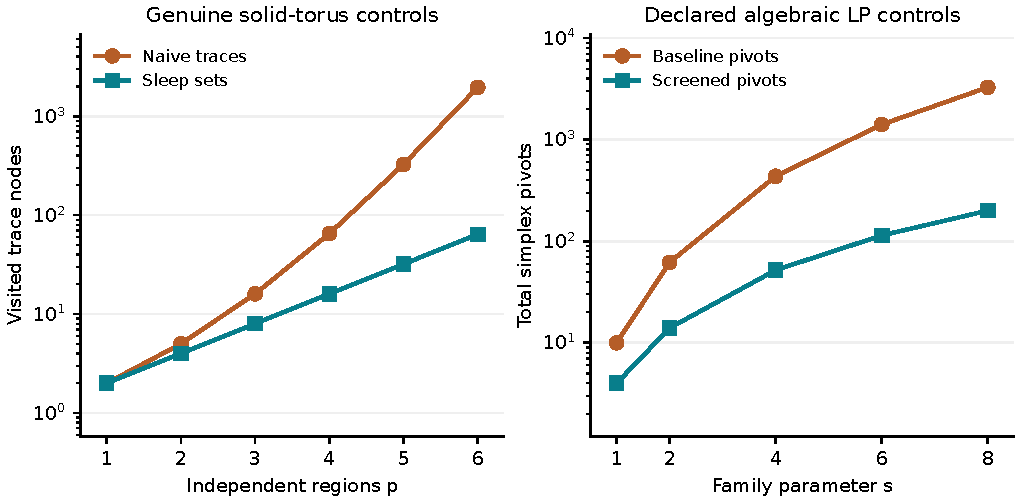
\includegraphics[width=\textwidth]{figures/performance.pdf}
\caption{Measured operation counts on the two controlled families. Left:
actual triangulations with independently collapsible regions, showing all
prefixes before and after sleep reduction. Right: the declared algebraic
LP family, showing exact total pivot counts. Logarithmic vertical axes are
used only for readability. Curves connect the tested integer sizes; the
formulas and their hypotheses, rather than these plots, establish the
asymptotic statements.}
\label{fig:performance}
\end{figure}

\subsection{What the evidence supports}

The geometric result is complete search of a declared finite move family,
with independent replay and a genuine example of factorial ordering
redundancy. The LP result is proof-preserving query omission, with moderate
genuine-triangulation gains and a stronger isolated algebraic separation.
The source adapter gives independently replayed positive diagram verdicts.
None of these observations establishes that every unknot has a successful
small-region trace, that every negative instance is settled by bounded
coherent search, or that exact node LPs have polynomial complexity.

The inherited and added regression tests are covered by the full inventory
gate described in Section~\ref{sec:reproduction}. The archive preserves its
logs, source digests and all failed or interrupted preliminary runs rather
than replacing them with the final successful summary.

\section{A concrete route toward quasi-polynomial recognition}\label{sec:research}

The locality theorem separates a search-theoretic cost that is now controlled
from geometric obligations that are not. This section states those obligations
as questions with testable intermediate targets. A change in a parameter or
source class should be reflected in the theorem statement, rather than hidden
inside an empirical success rate.

\subsection{The sufficient coverage theorem we would need}

Here is one precise form of a future global result. It allows a controlled
list of sources, rather than assuming that a single height seed works on
every diagram.

\begin{proposition}[Conditional recognition consequence]\label{prop:conditional}
Suppose there is an algorithm that, from an $n$-crossing knot diagram,
constructs at most $n^{O(\log n)}$ authenticated exterior triangulations with
specified integral cocycles and region budgets. Assume its construction
cost is $n^{O(\log n)}$, all source sizes and marking bit lengths are
polynomial in $n$, every region budget satisfies
$c=O(\log n)$ and $r+U=O(\log^2 n)$, and a complete component-disc predicate
has polynomial bit complexity on each resulting endpoint. Finally assume
the following uniform coverage property: every unknot diagram has a
compressing-disc endpoint in at least one of the resulting region families.
Then exhaustive region search gives an $n^{O(\log n)}$ unknot-recognition
algorithm.
\end{proposition}
\begin{proof}
Theorem~\ref{thm:local} bounds each search by $n^{O(\log n)}$; multiplying
by the number of sources preserves this bound. Source authentication and
component-disc replay make every positive verdict sound. The uniform
coverage property guarantees a positive endpoint on every unknot. Therefore,
after all the finite searches finish without one, the diagram is knotted.
The stated predicate cost ensures that this exhaustion is an algorithm,
not a search with unresolved endpoint queries.
\end{proof}

The proposition identifies exactly how a positive coverage theorem would
also justify negative decisions by exhaustion. No separate short negative
certificate is required for that logical consequence. The current artifact
does not establish uniform coverage and therefore does not take that final
negative step. A few short successful traces, or a coverage theorem only for
an already recognized subfamily of unknots, would be insufficient.

An alternative program can work through a certified hierarchy. In that case
one must bound the number, size and marking cost of all subsequent search
sources, as in \eqref{eq:outer-sum}, and prove the outer hierarchy complete.
A local simplification that can restart without a global decreasing measure
does not yet supply that bound.

\subsection{Priority 1: geometric locality and an honest obstruction search}

\paragraph{1. Which source families admit a logarithmic or squared-logarithmic region?}
Fix a concrete diagram-to-exterior construction, its shelling policy and
its cocycle normalization. Ask whether every solid torus in this source
family admits a disc endpoint with $r+U=O(\log^2 t)$, first with one connected
allowed region and then with $O(\log t)$ components. The theorem should
specify whether the cocycle is fixed, optimized by vertex potentials, or
selected from a bounded list. Changing that choice changes the coverage
problem.

A useful initial milestone is a proof for one explicit infinite family of
unknot diagrams that survives the existing shortcut stages and creates
nontrivial interior move choices. Merely testing a family whose initial
coherent seed is already a disc would establish little about geometric
search. The cancelled-braid empty-region miss and the eight-tetrahedron
obstruction are starting controls with different failure mechanisms.

\paragraph{2. Can the required region or upward budget be proved large?}
For increasing triangulated solid tori, compute the minimum allowed-region
size and minimum total upward count separately. Certified lower bounds
require complete exhaustion of the smaller family, with no capped endpoint
queries. Such computations can refute an overly strong conjecture on a
finite example, while a family construction could rule out a proposed
uniform logarithmic theorem. Useful adversarial sources include long layered
regions, separated interacting defects, and relabelled copies that expose
heuristics based on arbitrary row order.

The target is not to optimize a single scalar $r+U$ before understanding
both terms. A small permitted spatial region may still need many expansion
events, and a trace with few upward events can consume a large initial
region. The current count makes their different geometric meanings visible.

\paragraph{3. Can hierarchy structure produce the needed regions?}
Relate the initial consumption footprint to the product regions,
multi-surfaces and controlled decompositions in the hierarchy program
\cite{LackenbyTalk,Lackenby2026}. A useful lemma would take one precisely
specified reduction object, produce a legal marked trace, and bound its
consumed original cells, number of components and total expansions. The
proof must include the representation of the surface and its marking after
cutting. An existence theorem for a topological simplification without this
translation leaves the algorithmic parameters unbounded.

The successful reduction object may be much smaller than the normal surface
it encodes. Binary multiplicity is therefore compatible with a small region
theorem; enumerating all normal sheets to locate that region is not.
Conversely, the height-growth lemma alone controls arithmetic and gives
no spatial localization. These two estimates should be proved separately
and combined only at the final cost accounting.

\paragraph{4. Can small excess height be converted to a small total budget?}
Pachner-graph experiments often constrain maximum excess tetrahedron count
\cite{BurtonPachner}, whereas the theorem here constrains total upward
events. A conversion theorem would need to remove redundant excursions or
bound essential returns. Commuting disjoint moves removes order redundancy
but does not eliminate a sequence of dependent expansion--collapse cycles.
An exact state-based loop-removal argument may help with shortest traces;
its state count and marking dependence must be included. A bound on upward
bursts has the same issue and should not be substituted for $U$.

\subsection{Priority 2: stronger complete geometric search}

\paragraph{5. Can separators replace total active-region size?}
The commitment bound charges every freely assigned incarnation. In a long
trace whose interactions have a small separator, a dynamic program might
reuse completed subregions instead. A promising parameter is the width of
the dependency graph of events, with edges whenever one event consumes a
cell created or constrained by another. The first theorem needed is a
bounded interface description: which boundary face maps, local cocycle
values, surviving identities and surface data suffice to compose partial
traces? Without that description, invoking treewidth only renames the
state-explosion problem.

A concrete target is a family with $r=\Theta(t)$ but logarithmic interface
width, together with a finite compatibility relation and a proved state
count polynomial in the marking bit length. This would extend the useful
class beyond small initial footprints.

\paragraph{6. Which additional local relations safely reduce trace classes?}
The present sleep relation uses disjoint supports. Burton's overlapping
composite relations suggest larger reductions \cite{BurtonPachner}. Each
candidate needs a marked relative-boundary proof and an event-identity rule
that remains stable under other reductions. Test completeness against the
naive oracle before evaluating speed. A raw triangulation transposition table
must include remaining resources and continuation restrictions, or supply a
dominance proof. Equal unmarked endpoints alone do not justify dropping
one search state.

Region enumeration itself offers a modest immediate target: share exact
endpoint-predicate results across allowed regions while retaining separate
continuations. The proof should distinguish the terminal surface property,
which can be reused, from the permissions to consume original cells,
which differ. This avoids repeatedly checking the source endpoint and other
common states without changing the searched union.

\paragraph{7. Can the framework include the other Pachner moves?}
For unmarked formal star replacements, a tentative alphabet would have
six edge ports, four face ports, four vertex ports, one whole-cell port
and idle, for sixteen symbols. If $u_{23},u_{14}$ count expansions and
$d_{32},d_{41}$ count contractions, set $E=u_{23}+3u_{14}$. The tetrahedron
balance gives
\[
 d_{32}+3d_{41}\le t+E.
\]
The birth count then obeys
\[
 t+3u_{23}+4u_{14}+2d_{32}+d_{41}\le3t+5E.
\]
This accounting suggests an analogous constant-alphabet theorem, but the
formal-star legality, commutation and marking rules must be proved before
asserting it for an implementation. In particular, a $1$--$4$ move introduces
an interior vertex whose cocycle height needs a canonical choice or an
explicitly bounded search. The current artifact does not implement that
extension.

\paragraph{8. Can positive traces be made smaller without weakening replay?}
The explicit-snapshot certificate is polynomial for one bounded trace, but
repeats unchanged surrounding tetrahedra at every move. A persistent face-map
representation or a shared-prefix certificate DAG could remove that
duplication. The independent verifier should accept a stream of local changes,
check the same relative-boundary facts, and bound its memory. Storing all
endpoints of an exponential search is a different problem: a compact proof
of one success does not compress the whole search tree.

\subsection{Priority 3: exact LP discovery and normal-surface structure}

\paragraph{9. Can a genuine triangulation realize a superconstant screening gain?}
The algebraic separation has unit coefficients and sparse equations, but
normal matching matrices also encode very specific face and disc-type
incidences. Construct a family of actual compact triangulations for which
the ordered baseline makes asymptotically more deletion calls than local
witness screening. A weaker useful first target is a rigorous lower bound
on the number of redundant baseline tests in a layered or glued family,
with a matching positive point and independently checked topology. The
finite solid-torus timings do not establish such an asymptotic family.

\paragraph{10. What geometric hypotheses bound the support antichain?}
Proposition~\ref{prop:exponential-antichain} rules out a small-antichain
argument from sparsity and unit coefficients alone. Possible additional
hypotheses include a controlled decomposition of the triangulation, a
bounded number of quad types interacting with the boundary, or a restricted
rank-one cone. The desired theorem should bound the number of useful
minimal supports or provide a small subcollection covering all deletion
queries encountered by a specified branch policy. Bounding all supports
may be stronger than the algorithm needs.

\paragraph{11. Can first-node LPs be accelerated with exact dual lifting?}
The capped figure-eight controls make this a direct implementation priority.
An equality-row basis can reduce a redundant matrix before simplex. A
certificate of the row transformation allows a dual of the reduced problem
to be lifted to the original equations. Fraction-free elimination and sparse
factorization are natural candidates, but their exact coefficient growth,
per-mask rank changes and reconstruction cost need measurements and proofs.

Such an optimization can preserve mathematical soundness while changing
the exact serialized multiplier and hence falls outside the byte-preserving
mode proved here. It should have its own compatibility contract. More
ambitiously, a polynomial-bit-complexity LP method can replace the pivot
engine while retaining exact independently checked primal or dual outputs;
one must count its recovery and verification work, not merely invoke a
real-arithmetic LP bound. Warm starts are another practical direction,
but need careful basis validation after coordinates are deleted.

\paragraph{12. How should positive and negative evidence interact?}
Positive supports safely answer any further zero restriction containing
them. A negative dual has the opposite issue when columns are restored:
its inequality must be checked on every newly allowed column. A two-sided
cache could reuse both forms of evidence with full matrix checks. Its
branch policy and final proof may change, so compare it against the present
byte-preserving producer rather than silently weakening that guarantee.
Useful quantities include exact validation cost, cache hit location, and
the number of current-node LPs avoided.

\paragraph{13. Can propagation backdoors be bounded after geometric preprocessing?}
The incoming dual-certificate work isolates quadrilateral propagation
backdoors. The locality search may expose triangulations with smaller
backdoors even when it does not directly find a disc. A joint theorem
would bound both the cost of reaching such a triangulation and the number
of unresolved choices afterwards. The endpoint predicate would then be
algebraic complexity reduction rather than immediate disc discovery. It
must remain source-bound, and the outer choice of endpoints must not
reintroduce an uncontrolled number of LP searches.

\subsection{Priority 4: evaluation that can disprove the proposed story}

\paragraph{14. What does a matched source-level cohort show?}
Create a frozen cohort stratified by original diagram crossings, exterior
tetrahedron count, known shortcut success and initial coherent-disc status.
Every arm should receive identical face pairings and marking choices.
Compare time to a verified positive or negative result, the proportion
remaining inconclusive under explicit caps, total upward moves, region size,
endpoint-query time, LP pivots and certificate size. Independent relabellings
and matched constructor versions are essential controls for order-sensitive
heuristics. The present fifteen LP cases and six geometric control sizes
are useful mechanism tests, not such a representative recognition study.

\paragraph{15. Which empirical claims survive fixed-resource reproduction?}
Repeat paired timing in an isolated environment, report all censored runs,
and retain the raw per-pair observations. Separate source construction,
search, terminal verification and later independent replay when their cost
matters. A speedup that disappears after including required verification is
not an end-to-end gain. A future benchmark should also include the unfavorable
small cases and node-LP bottlenecks already observed here.

The highest-value next result is a geometric theorem bounding the parameters
in Proposition~\ref{prop:conditional}, or a rigorous obstruction showing
that a proposed bound fails. The next implementation result is exact
current-node LP acceleration with a checked reconstruction map. Both have
clear acceptance criteria and address limitations that the present proofs
and experiments identify directly.

\section{Reproduction, provenance and integration}\label{sec:reproduction}

\subsection{Archive organization}

The ZIP is designed to be both a readable research record and an additive
integration proposal. Its root directory contains the report sources and
compiled PDF, a runnable source snapshot, raw evidence and an integration
tool. The file manifest records byte lengths and SHA-256 digests. The
integration manifest additionally identifies which additions come from the
earlier incoming packages and which are introduced by this continuation.

\begin{center}
\small
\begin{tabularx}{\textwidth}{@{}lX@{}}
\toprule
Location & Contents\\
\midrule
\path{article/} & Main TeX, section sources, bibliography, generated tables, figure PDF/PNG and compiled article\\
\path{repro/fast/} & Pinned fast tree plus dependency additions and the five new runtime modules; tests and research drivers\\
\path{repro/reports/}, \path{repro/synthesis/} & Exact historical reference modules and fixtures needed by inherited tests\\
\path{integration/} & Dependency and new-work overlays, code-review patch, preflight/apply tool and origin manifest\\
\path{provenance/} & Pinned source digests, incoming archive digests, integration audit and complete regression logs\\
\path{scripts/} & Evidence-table/figure regeneration and package integrity verification\\
\path{README.md} & Entry points, dependency notes, theorem scope and reproduction commands\\
\bottomrule
\end{tabularx}
\end{center}

The source snapshot avoids a dependency on the current GitHub main branch.
The external mathematical literature is cited by stable versions or precise
document URLs. Full third-party papers are not copied into the archive.
The three prior incoming archives remain identified by their repository
paths and immutable Git objects; the executable additions needed from them
are included directly.

\subsection{Run the new focused tests}

The new runtime code uses the Python standard library. The optional topology
cross-check uses Regina. Plot regeneration additionally uses Matplotlib;
building the report uses a normal \LaTeX{} installation with the listed
packages. Python 3.12.14 and Regina 7.4 describe the recorded execution, not
a promise that every other version gives identical timings or simplex
implementation behavior after source changes.

From \path{repro/fast/}:

\begin{lstlisting}
python -m unittest \
  tests.test_pachner_commitments \
  tests.test_pachner_regions \
  tests.test_normal_pachner_search \
  tests.test_normal_propagation_cached -v
\end{lstlisting}

These four modules contain 29 new tests. The inherited test suite is much
larger and includes historical reference imports outside \path{fast/};
the supplied companion directories preserve those relative paths.

\subsection{Replay saved evidence before rerunning timings}

The following commands independently replay the saved geometric and
source-bound evidence. They do not rerun the expensive benchmark search.

\begin{lstlisting}
python -m commitment_research.run replay \
  --input commitment_research/results/audit.json \
  --output commitment_research/results/reproduced_audit_replay.json
python -m commitment_research.run replay \
  --input commitment_research/results/benchmark.json \
  --output commitment_research/results/reproduced_benchmark_replay.json
python -m region_research.audit \
  --replay region_research/results/audit.json \
  --output region_research/results/reproduced_replay.json
\end{lstlisting}

The LP evidence has a separate verifier-only command:

\begin{lstlisting}
python -m lp_cache_research.replay \
  --output lp_cache_research/reproduced_replay.json
\end{lstlisting}

It independently checks all seven distinct completed genuine certificates,
42 paired-sample certificate-digest references and ten genuine source
digests. It reconciles all fifteen summary rows, but excludes the three
inconclusive genuine cases and five algebraic certificates from geometric
certificate replay. No search, LP solver or native constructor is imported.
The focused cache test suite repeats the positive, negative and policy
controls. The algebraic harness intentionally substitutes model construction
and final analysis; its certificates must not be passed off as geometric
normal-surface certificates.

To reconstruct the finite audits and paired measurements:

\begin{lstlisting}
python -m commitment_research.run audit \
  --output commitment_research/results/reproduced_audit.json
python -m commitment_research.run benchmark --repeats 3 \
  --output commitment_research/results/reproduced_benchmark.json
python -m region_research.audit \
  --output region_research/results/reproduced_audit.json
python -m lp_cache_research.audit --rounds 3 --timeout 35 \
  --figure-pivots 600 --output lp_cache_research/reproduced_results.json
\end{lstlisting}

The optional external move inventory check is documented in
\path{commitment_research/README.md}. It requires Regina and compares
exact source and target triangulations. Replaying a saved file and
regenerating a constructor-dependent fixture are different tasks, and the
drivers retain that distinction.

\subsection{The complete regression gate}

The final gate covers the complete inventory of test modules under the
combined fast tree. It uses six fresh Python processes with each module
assigned exactly once; the machine-readable record lists module and test
identities, source digests, counts, statuses and per-batch logs. This avoids
depending on a single long-lived process for a suite with many historical
and optional native-library tests.

\begin{table}[tbp]
\centering
\small
\setlength{\tabcolsep}{4pt}
\caption{Complete final regression gate. Each test module belongs to one selected passing batch.}
\label{tab:regression}
\begin{tabular}{@{}rrrrl@{}}
\toprule
Batch & Modules & Tests & Seconds & Result\\
\midrule
1 & 31 & 227 & 59.898 & PASS\\
2 & 30 & 221 & 38.288 & PASS\\
3 & 30 & 280 & 21.664 & PASS\\
4 & 30 & 238 & 35.743 & PASS\\
5 & 30 & 256 & 28.164 & PASS\\
6 & 30 & 215 & 17.531 & PASS\\
\midrule Total & 181 & 1,437 & 201.289 & PASS\\
\bottomrule
\end{tabular}
\par\smallskip
\begin{minipage}{0.97\textwidth}
\footnotesize Zero failures, errors or skips in the final selected batches; zero module omissions. The preliminary interrupted run and the corrected native-fixture test failure are preserved separately.
\end{minipage}
\end{table}


The preliminary history is retained. An initial single-process discovery
run encountered omitted historical companion files and later ended without
a normal unittest summary. Those files were restored byte-for-byte from
the pinned revision. A focused retry of the affected modules passed.
During the complete inventory run, one newly added optional test incorrectly
required a freshly simplified Regina figure-eight exterior to equal a
particular frozen triangulation. The test was corrected to validate each
source against its own construction or saved record. The affected batch
was then rerun; its initial failure and corrected source digest remain in
the provenance. The producer, baseline LP engine and benchmarks were not
changed to resolve that test assumption.

The passing gate is therefore a claim about a precise final source snapshot,
not a claim that every preliminary run passed. Source hashes also make
clear which post-measurement edits only improved documentation.
The portable \path{scripts/rerun_regression.py} lists the exact partition by
default and repeats it with \code{--run}, writing fresh logs without replacing
the recorded evidence.

\subsection{Apply the proposed additions}

The integration tool preflights every target path and baseline prerequisite
before creating any files. It accepts an existing addition only when its
bytes are identical, refuses conflicting content and performs no replacement
of a maintained file. It defaults to a review operation; the explicit apply
option creates the missing additions. From the archive root:

\begin{lstlisting}
python integration/apply_overlay.py --repo /path/to/ProveIt --check
python integration/apply_overlay.py --repo /path/to/ProveIt --apply
\end{lstlisting}

The pinned-revision check and the prerequisite digests prevent an apparently
successful integration against incompatible source APIs. A later repository
revision should be reviewed explicitly, rather than patched by relaxing a
digest mismatch. The full overlay includes reproducibility material;
the code-review patch is a convenient view of Python changes, not a substitute
for the dependency and evidence layers.

The packaging audit applies the additions to a clean local copy of the
pinned fast source, checks all resulting file hashes, confirms that no
maintained source bytes changed, and checks a second application for
idempotence. It does not publish or push anything to GitHub.

\subsection{Rebuild and verify the report}

From the archive root, first verify the shipped bytes, then regenerate
the tables and figure from the saved measurements and compile:

\begin{lstlisting}
python scripts/verify_manifest.py
python scripts/build_evidence.py
latexmk -pdf -interaction=nonstopmode -halt-on-error \
  -cd article/article.tex
\end{lstlisting}

The shipped PDF was compiled with resolved citations and references, then
rendered page by page for visual inspection. The generated plots use the
recorded integer operation counts and clearly distinguish genuine
triangulations from the algebraic control. Recompilation can change PDF
metadata or engine-dependent byte layout; the integrity manifest authenticates
the shipped bytes, not every future rebuild of equivalent content.

\appendix
\section{Exact pivot counts for the algebraic screening family}
\label{sec:pivot-appendix}

The oracle-call separation in Theorem~\ref{thm:lp-family} can be strengthened
for the exact simplex implementation supplied with the repository. This
appendix proves the pivot counts, including the entering and leaving choices;
it does not infer them from the experimental table. The statement concerns
the algebraic family~\eqref{eq:lp-family}, with its specified ordering and
solver. No realization by three-manifold triangulations is asserted.

\begin{theorem}[Exact pivot separation]\label{thm:lp-pivots}
For the $s$-block algebraic family of Theorem~\ref{thm:lp-family}, run the
specified all-slack Bland solver without a pivot cutoff, or with an allowance
sufficient for both complete propagation runs. The total numbers of simplex
pivots are
\begin{equation}\label{eq:lp-pivot-counts}
 P_{\rm base}(s)=6s^3+3s^2+s,
 \qquad
 P_{\rm screened}(s)=3s^2+s.
\end{equation}
Every positive current-node or irrelevant-coordinate deletion query uses
exactly $2s$ pivots. Deleting the mandatory type-zero coordinate of block
$j$, where $0\le j<s$, uses exactly $2j$ pivots. Global cache capacity zero
suffices for the screened formula.
\end{theorem}

We first establish a tableau lemma that includes all the restrictions
arising during these propagation runs.

\subsection{Ordered chain systems and the exact initial tableau}

Let $m\ge1$. Consider disjoint groups $G_0,\ldots,G_{m-1}$ of nonnegative
original variables, none containing a distinguished variable $z$. A group
may contain several variables with identical columns, or it may be empty.
Write
\[
 X_i=\sum_{x\in G_i}x.
\]
Let $\mathcal Y$ contain all other original variables, whose matching
columns and objective coefficients are zero, and put
$Y=\sum_{y\in\mathcal Y}y$. The matching equations, in this exact order,
and the objective are
\begin{equation}\label{eq:pivot-chain}
 X_i-z=0\quad(0\le i<m),\qquad \text{objective }z.
\end{equation}
The normalization used by the solver is
\begin{equation}\label{eq:pivot-normalization}
 z+\sum_{i=0}^{m-1}X_i+Y\le1.
\end{equation}

The implementation forms the inequalities $Cx\le0$, followed by
$-Cx\le0$, followed by~\eqref{eq:pivot-normalization}. It adds one
nonnegative slack to each row and starts with the all-slack feasible basis.
Denote the slacks of the $C$ rows by $a_0,\ldots,a_{m-1}$, those of the
$-C$ rows by $b_0,\ldots,b_{m-1}$, and the normalization slack by $\sigma$.
Thus the initial tableau equations are
\begin{align}
 a_i+X_i-z&=0 &&(0\le i<m),\label{eq:pivot-initial-plus}\\
 b_i-X_i+z&=0 &&(0\le i<m),\label{eq:pivot-initial-minus}\\
 \sigma+z+\sum_{i=0}^{m-1}X_i+Y&=1.\label{eq:pivot-initial-sum}
\end{align}
Every original variable precedes every slack in the variable order.
Slack indices then follow the displayed row order: all $a_i$, all $b_i$,
then $\sigma$. Removing an original column preserves the relative order
of the remaining original variables and of all the slacks.

The entering rule chooses the least-index variable with strictly positive
reduced objective coefficient. The leaving rule minimizes the usual
nonnegative ratio and, among equal ratios, chooses the least-index current
basic variable. Zero reduced coefficients are never selected. The solver
returns immediately once the objective is positive, or when no positive
reduced coefficient remains.

\begin{lemma}[Exact chain pivot path]\label{lem:pivot-chain}
Assume $z$ is present. If every $G_i$ is nonempty, the solver for
\eqref{eq:pivot-chain} returns a positive point after exactly $m+1$ pivots.
If $h$ is the first index for which $G_h$ is empty, it returns a nonpositive
certificate after exactly $h+1$ pivots. These assertions are independent
of the number of irrelevant variables and of the number of available
duplicate columns in each nonempty group.
\end{lemma}
\begin{proof}
Initially $z$ is the only variable with positive reduced coefficient.
Its coefficients are $-1$ in the $C$ rows, $+1$ in the $-C$ rows, and
$+1$ in the normalization row. All $-C$ rows have ratio zero, whereas
the normalization row has ratio one. The leaving variable is therefore
$b_0$, by the specified slack ordering and Bland tie rule. The pivot
coefficient is one, the objective remains zero, and the resulting
dictionary expresses
\[
 z=X_0-b_0.
\]

Here is the full inductive invariant. After $h+1$ pivots, suppose that
$G_0,\ldots,G_{h-1}$ were nonempty. Let $x_i$ be the least-index available
member of $G_i$ that entered for $i<h$, and put $Y_i=X_i-x_i$.
The basic original variables are $z,x_0,\ldots,x_{h-1}$. All $a_i$, all
$b_j$ with $j>h$, and $\sigma$ are also basic. The nonbasic slacks are
$b_0,\ldots,b_h$. The tableau equations are exactly
\begin{align}
 z-X_h+b_h&=0,\label{eq:pivot-invariant-z}\\
 x_i+Y_i-X_h+b_h-b_i&=0 &&(i<h),\label{eq:pivot-invariant-old}\\
 a_i+b_i&=0 &&(i\le h),\label{eq:pivot-invariant-completed}\\
 a_j+X_j-X_h+b_h&=0 &&(j>h),\label{eq:pivot-invariant-plus}\\
 b_j-X_j+X_h-b_h&=0 &&(j>h),\label{eq:pivot-invariant-minus}\\
 \sigma+(h+2)X_h-(h+1)b_h
       +\sum_{i<h}b_i+\sum_{j>h}X_j+Y&=1.
       \label{eq:pivot-invariant-normalization}
\end{align}
The current objective value is zero, and its reduced expression is
\begin{equation}\label{eq:pivot-reduced}
 z=X_h-b_h.
\end{equation}
All tableau right-hand sides except that of the normalization row are
zero. Direct elimination in~\eqref{eq:pivot-initial-plus}--
\eqref{eq:pivot-initial-sum} proves the invariant for $h=0$.

If $G_h$ is empty, equation~\eqref{eq:pivot-reduced} has no positive
reduced coefficient: $b_h$ has coefficient $-1$, and all other nonbasic
variables have coefficient zero. The solver therefore stops after
$h+1$ pivots with its nonpositive certificate.

Suppose instead that $G_h$ is nonempty. Precisely its variables have
positive reduced coefficient, each equal to one. Bland consequently
selects $x_h=\min G_h$. Its coefficient is $-1$ in the $z$ row and in
each earlier $x_i$ row, zero in the $a_i$ rows with $i\le h$, $-1$ in
the later $a_j$ rows, $+1$ in the later $b_j$ rows, and $h+2$ in the
normalization row. Thus the only eligible leaving rows are the later
$b_j$ rows, with ratio zero, and normalization, with ratio $1/(h+2)$.

If $h<m-1$, a zero-ratio row exists. The remaining basic variables
$b_j$, $j>h$, retain their original indices, so Bland chooses $b_{h+1}$.
This is a unit pivot in a row with zero right-hand side. Substitution
using
\[
 X_h=X_{h+1}-b_{h+1}+b_h
\]
gives every invariant equation with $h$ replaced by $h+1$; the new basic
variable $x_h$ supplies the additional instance of
\eqref{eq:pivot-invariant-old}. The normalization coefficients become
$h+3$ and $-(h+2)$, as required. The objective is still zero. This
establishes the induction, including both Bland choices.

If $h=m-1$, there is no later $b_j$ row. The only eligible leaving row
is normalization, with pivot coefficient $m+1$. This final pivot sets
$x_{m-1}=1/(m+1)$ and makes the objective $1/(m+1)>0$.
The implementation returns immediately. The initial $z$ pivot and the
$m$ entering-group pivots give exactly $m+1$ pivots.

Throughout the zero-objective stages, irrelevant variables have zero
reduced coefficient by~\eqref{eq:pivot-reduced}, so none enters.
If a group has several available twins, all have the same positive
coefficient when that group is current and Bland selects its least member.
Afterwards its other twins have reduced coefficient zero. If an earlier
twin was already forbidden before the LP call, the least remaining
member is selected instead. These observations prove the asserted
independence from irrelevant columns and available multiplicities.
\end{proof}

\begin{lemma}[Deletion of the objective variable]\label{lem:pivot-zero-objective}
If the column $z$ is deleted from the restricted query, the solver returns
its nonpositive certificate with zero pivots.
\end{lemma}
\begin{proof}
All remaining original objective coefficients are zero, as are the initial
slack coefficients. The all-slack objective value is zero and there is no
entering variable. The stopping test precedes any pivot.
\end{proof}

\subsection{The actual block ordering and previous propagations}

For the family~\eqref{eq:lp-family}, put $m=2s-1$. The exact matching-row
order used by the model builder is
\begin{align*}
 (Cx)_0&=q_{0,1}+p_0-z,\\
 (Cx)_{2j-1}&=q_{j,0}-z &&(1\le j<s),\\
 (Cx)_{2j}&=q_{j,1}+p_j-z &&(1\le j<s).
\end{align*}
Equivalently, the chain groups before propagation are
\begin{align*}
 G_0&=\{q_{0,1},p_0\},\\
 G_{2j-1}&=\{q_{j,0}\} &&(1\le j<s),\\
 G_{2j}&=\{q_{j,1},p_j\} &&(1\le j<s).
\end{align*}
For completeness, let $n_s=7(2s+\lceil s/4\rceil)$ and index the original
columns $v_0,\ldots,v_{n_s-1}$ in increasing order. In each seven-coordinate
block, the four triangle coordinates precede the three quadrilateral
coordinates. With zero-based indices, the distinguished columns are
\begin{align*}
 q_{j,0}&=v_{7(s+j)+4},&
 q_{j,1}&=v_{7(s+j)+5} &&(0\le j<s),\\
 p_j&=v_{14s+7\lfloor j/4\rfloor+(j\bmod4)}
 &&&&(0\le j<s).
\end{align*}
Thus $z=v_{7s+4}$, and every $q_{j,1}$ precedes its auxiliary triangle
twin $p_j$. These are the block and column conventions of
Section~\ref{sec:witness}. All remaining variables are irrelevant
variables of the chain lemma. The synthetic model has no triangle-anchor
restrictions.

At propagation stage $j$, each earlier block $\ell<j$ has been forced to
quadrilateral type zero. Its variable $q_{\ell,1}$ has therefore been
removed, while $p_\ell$ remains available. Its group $G_{2\ell}$ becomes
the nonempty singleton $\{p_\ell\}$. All other row groups remain nonempty.
Lemma~\ref{lem:pivot-chain} consequently gives exactly
$m+1=2s$ pivots for every current-node LP.

Deleting a tested irrelevant prefix coordinate removes only one member of
$\mathcal Y$. It neither changes the objective nor empties a row group,
so every such deletion query also takes exactly $2s$ pivots. Although the
number of restricted original columns changes, the relative slack order
used in the leaving-variable proof does not.

Deleting the mandatory coordinate $q_{j,0}$ has two different cases.
For $j=0$, this is deletion of $z$, so
Lemma~\ref{lem:pivot-zero-objective} gives zero pivots. For $j>0$, it
empties $G_{2j-1}$ and leaves all earlier groups nonempty. The first empty
row is thus $h=2j-1$, and Lemma~\ref{lem:pivot-chain} gives
$h+1=2j$ pivots.

\subsection{Summing the exact costs}

\begin{proof}[Proof of Theorem~\ref{thm:lp-pivots}]
Theorem~\ref{thm:lp-family} establishes that both runs make $s+1$
current-node queries and $s$ mandatory deletion queries. The former
each cost $2s$ pivots, and the latter cost $0,2,\ldots,2(s-1)$.
The baseline additionally makes $3s^2$ positive irrelevant-prefix
deletion queries, each costing $2s$ pivots. Hence
\begin{align*}
 P_{\rm base}(s)
   &=(s+1)(2s)+(3s^2)(2s)+\sum_{j=0}^{s-1}2j
     =6s^3+3s^2+s,\\
 P_{\rm screened}(s)
   &=(s+1)(2s)+\sum_{j=0}^{s-1}2j
     =3s^2+s.
\end{align*}
Screening these particular deletions needs only the current-node witness,
so a zero-capacity persistent cache gives the same result.
\end{proof}

The difference is exactly $6s^3$ pivots. The proof concerns the specified
matrix family, column and row orders, strict entering rule, and stopping
tests. It establishes neither a polynomial pivot bound for arbitrary
Bland-simplex inputs nor a universal wall-clock factor. It also leaves
the separate geometric realizability question unchanged.

\section{Claim and assumption ledger}\label{sec:ledger}

This ledger makes the boundary of each result explicit for repository
integration and later mathematical review.

\begingroup\small
\begin{longtable}{@{}>{\raggedright\arraybackslash}p{0.22\textwidth}>{\raggedright\arraybackslash}p{0.37\textwidth}>{\raggedright\arraybackslash}p{0.34\textwidth}@{}}
\toprule
Claim & Required assumptions & Evidence or proof boundary\\
\midrule
\endfirsthead
\toprule
Claim & Required assumptions & Evidence or proof boundary\\
\midrule
\endhead
Disjoint local moves commute & Simultaneously legal repository-style formal bipyramid replacements with disjoint consumed cells & Lemma~\ref{lem:commute}; tracked boundary maps and cocycles; no strict-simplicial extension claimed\\[0.45em]
Constant-alphabet encoding & At most $U$ total upward moves; exact incarnation ports & Theorem~\ref{thm:commitment}; $11^{3t+5U}$, or $7^{3t}$ downward\\[0.45em]
Sleep search has the same count & Exact birth identities, canonical local frames, dynamic persistence of enabled independent events & Theorem~\ref{thm:sleep}; continuation states are not merged by endpoint equality\\[0.45em]
Region-sensitive search & Consumed initial footprint contained in an allowed $r$-cell region with at most $c$ components & Theorem~\ref{thm:local}; constructive enumeration; actual footprint can have more components than its cover\\[0.45em]
Quasi-polynomial search class & $c=O(\log t)$, $r+U=O(\log^2t)$; polynomial complete endpoint predicate & Corollary~\ref{cor:quasi}; no universal coverage of unknots supplied\\[0.45em]
Binary marking control & Prescribed relative-boundary height transport & Lemma~\ref{lem:bits}; $B+U+O(1)$ bits; component-predicate cost remains explicit\\[0.45em]
Diagram-bound positive verdict & Authenticated exterior, replayed changes and an independently verified essential-disc component & Existing unchanged diagram verifier; every nonpositive bounded outcome is inconclusive\\[0.45em]
Exact LP certificate preservation & Fixed deterministic engine/policy; full support validation; no external time/callback cutoff for budget comparison & Theorem~\ref{thm:lp-policy}; node/depth/pivot completion preservation\\[0.45em]
Support-sensitive sweep & Pinned verified current witness, even with persistent cache capacity zero & Corollary~\ref{cor:lp-support}; does not bound number of branch nodes\\[0.45em]
Exponential support antichain & Declared sparse algebraic cone & Proposition~\ref{prop:exponential-antichain}; no triangulation realization needed for the algebraic limitation\\[0.45em]
Quadratic-to-linear LP calls & Explicit seven-block model and original column order & Theorem~\ref{thm:lp-family}; $3s^2+2s+1$ versus $2s+1$\\[0.45em]
Cubic-to-quadratic pivots & Same model plus the exact ordered all-slack Bland tableau and stopping rule & Theorem~\ref{thm:lp-pivots}; full induction; not a general bit-time theorem\\[0.45em]
Measured geometric speedup & Six declared inverse-bipyramid controls and three recorded pairs per size & Raw source/certificate/timing files; $22.18$ paired ratio at $p=6$; small case regression retained\\[0.45em]
Measured LP improvement & Fifteen declared cases, matched sources and explicit resource caps & Completed genuine certificates independently replay; figure-eight runs remain inconclusive\\[0.45em]
General quasi-polynomial recognition & Uniform source construction and coverage hypotheses of Proposition~\ref{prop:conditional} & Conditional consequence only; this article does not prove those hypotheses\\
\bottomrule
\end{longtable}
\endgroup

\subsection{Useful counterexamples to tempting shortcuts}

The following examples delimit the mechanisms rather than merely lowering
reported success rates.

\begin{enumerate}
\item A coherent disc can transport to a disc plus spheres. Therefore total
Euler characteristic and preserved cohomology do not certify preserved
surface topology.
\item A surviving tetrahedron can change row number after a disjoint move.
Therefore row-number action identities are not stable enough for sleep
pruning or birth-name equivalence.
\item An event can consume the output of a previous event while their
consumed input sets are disjoint. Therefore historical input disjointness
is not by itself a static independence relation.
\item Two equal endpoint triangulations can carry different remaining
upward budgets or sleep restrictions. Therefore endpoint-query deduplication
does not authorize merging their continuations.
\item A positive witness valid under one triangle anchor can violate another
anchor. Therefore checking only its tested quadrilateral coordinate is
insufficient for cross-query reuse.
\item A sparse unit-coefficient cone can have $2^k$ minimal positive supports.
Therefore an unlimited witness antichain is not automatically polynomial.
\item The cancelled-braid unknot can exhaust the tested empty-region family
without a disc certificate. Therefore finite-family exhaustion is not an
unconditional negative knot verdict.
\item Native simplification can yield different finite triangulations of
the same manifold. Therefore a fresh construction should not be required
to equal a saved combinatorial fixture unless determinism has been proved.
\end{enumerate}

\subsection{Research status}

The explicit proofs received separate internal mathematical and implementation
reviews. The finite audit uses independent replay and an optional external
topology oracle. This report and its code were prepared with AI assistance
for ProveIt and are submitted for external mathematical and code review.

\clearpage
\begingroup\small\raggedright
\setlength{\parskip}{0pt}
\bibliographystyle{plain}
\bibliography{references}
\endgroup
\end{document}
